\documentclass[preprint, 10pt]{elsarticle}

\newcommand{\mcaption}[2]{\caption{\small \em #1}\label{#2}}
\newcommand{\secref}[1]{\ref{#1}}

%\usepackage{algorithmic}
%\usepackage{algorithm}
\usepackage{amsfonts}
\usepackage[fleqn,reqno]{amsmath}
\usepackage{amssymb}
%\usepackage{amsthm}
\usepackage[titletoc]{appendix}
\usepackage{array}
%\usepackage{bm}
%\usepackage{caption}
%\usepackage[usenames]{color}
\usepackage{enumitem}
%\usepackage{epsfig}
%\usepackage{fancybox}
\usepackage{filecontents}
\usepackage[top=1.2in,bottom=1.2in,left=1in, right=1in]{geometry}
\usepackage{graphics}
%%\usepackage{ifthen}
\usepackage{lineno}
%\usepackage{mathrsfs}
%\usepackage{mdframed}
%\usepackage{multirow}
%\usepackage{palatino}
%\usepackage{showkeys} %To see the labels for now.  Will remove later
%\usepackage{stmaryrd}
%\usepackage{subfigure}
%\usepackage{paralist}
\usepackage{pgfplots}
%\usepackage{tabularx}
\usepackage{tikz}
\usepackage{todonotes}
\usetikzlibrary{arrows}
\usepackage{comment}

%%%%%%  pdftex  %%%%%%%%%%%%%%%%%%%%%%%%%%%%%%%%%%%%%%%%%%%%%%%%%%%%%%
\usepackage[pagebackref=false,bookmarks=false]{hyperref} 

\hypersetup{
  bookmarksnumbered=true,
  bookmarksopen=false,
  hypertexnames=false,      
  breaklinks=true,          
  unicode=false,
  pdffitwindow=true,        
  pdfnewwindow=true,        
  colorlinks=true,         
  linkcolor=dblue,
  anchorcolor=red,
  citecolor=dorange,
  filecolor=magenta,
  urlcolor=dblue,
  pdfstartview = FitH,
  pdfkeywords = {},
  pdfcreator = {LaTeX with hyperref package}
}



\newcommand{\bd}{{\partial}}
\newcommand{\bigO}{{\mathcal{O}}}
\newcommand{\cc}{{\mathbf{c}}}
\newcommand{\DD}{{\mathcal{D}}}
\newcommand{\eeta}{{\boldsymbol\eta}}
\newcommand{\ff}{{\mathbf{f}}}
\newcommand{\grad}{{\nabla}}
\newcommand{\II}{{\mathbf{I}}}
\newcommand{\iin}{\mathrm{in}}
\newcommand{\llambda}{{\boldsymbol\lambda}}
\newcommand{\nn}{{\mathbf{n}}}
\newcommand{\NN}{{\mathcal{N}}}
\newcommand{\out}{\mathrm{out}}
\newcommand{\rr}{{\mathbf{r}}}
\newcommand{\RR}{{\mathbb{R}}}
\renewcommand{\ss}{{\mathbf{s}}}
\newcommand{\ssigma}{{\boldsymbol\sigma}}
\newcommand{\tar}{\mathrm{tar}}
\newcommand{\uu}{{\mathbf{u}}}
\newcommand{\UU}{{\mathbf{U}}}
\newcommand{\vv}{{\mathbf{v}}}
\newcommand{\xx}{{\mathbf{x}}}
\newcommand{\xxi}{{\boldsymbol{\xi}}}
\newcommand{\yy}{{\mathbf{y}}}

\def\gap{\hspace*{.2in}}

% Derivatives
\newcommand{\pderiv}[2]{\frac{\partial #1}{\partial #2}}
\newcommand{\tderiv}[2]{\frac{d #1}{d #2}}
\newcommand{\ppd}[2]{\frac{\partial^2 #1}{{\partial #2}^2}}

% Nick's commands
\newcommand{\vsp}[1]{\vspace{#1 pc} \noindent}
\newcommand{\abs}[1]{\lvert #1 \rvert}
\newcommand{\mean}[1]{\left< #1 \right>}
\newcommand{\thL}{$\theta$--$L$}
\newcommand{\eps}{\varepsilon}
\newcommand{\Vn}{V_n}
\newcommand{\Vs}{V_s}
\newcommand{\atau}{\abs{\tau}}
\newcommand{\thalpha}{\pderiv{\theta}{\alpha}}
\newcommand{\elfun}{\zeta}
\newcommand{\thhat}{\hat{\theta}}
\newcommand{\Dt}{\Delta t}
\newcommand{\NLterm}{\mathcal{N}}
\newcommand{\Mterm}{\mathcal{M}}
\newcommand{\FourierSum}{ \sum_{k = -N_\iin /2}^{N_\iin /2-1} }
\newcommand{\atausig}{\atau^{(\sigma)}}
\newcommand{\Vnsig}{\Vn^{(\sigma)}}
\newcommand{\Vssig}{\Vs^{(\sigma)}}


\newcommand{\tauD}[1]{\tau_{#1\text{D}}}
\newcommand{\atauD}[1]{\abs{\tau_{#1\text{D}}}}

\begin{document}

\title{Viscous Erosion in Porous Media}

% OTHER TITLE POSSIBILITIES
% A fast and accurate method for viscous erosion in a 2D porous medium

\author[Bryan]{Bryan D.~Quaife}
\author[Nick]{M.~Nicholas J.~Moore}
\address[Nick]{Department of Mathematics and Geophysical Fluid Dynamics Institute, Florida State University, Tallahassee, FL, 32306.}
\address[Bryan]{Department of Scientific Computing and Geophysical Fluid Dynamics Institute, Florida State University, Tallahassee, FL, 32306.}

\begin{abstract} 
We develop numerical methods to simulate the fluid-mechanical erosion of
many bodies in a two-dimensional Stokes flow. The broad aim
is to simulate the erosion of a porous medium (e.g.~ground water flow)
with grain-scale resolution. Our fluid solver is based on a
second-kind boundary integral formulation of the Stokes equations that is
discretized with a spectrally-accurate Nystr\"om method and solved
with a fast-multipole-accelerated GMRES iteration. To evolve the individual grains under shear-driven
erosion, we regularize via curvature-penalization and solve the
associated system using the {\thL} formulation. This framework allows
numerically stable treatment of stiff terms, thus permitting large time
steps. The overall accuracy of our method is exponential in space and
second-order in time. The method is computationally efficient, with the
fluid solver requiring $\mathcal{O}(N)$ operations per GMRES iteration,
a mesh-independent number of GMRES iterations, and a one-time
$\mathcal{O}(N^2)$ computation to compute the shear stress. We benchmark single-body results against analytical predictions. In our multi-body simulations, we find that erosion leads to spontaneous channelization between bodies in near contact. The channelization is associated with a dramatic reduction in the resistance of the porous medium, much more than would be expected from the reduction in grain size alone.
\end{abstract}

\begin{keyword}
  Porous medium \sep Stokes flow \sep Erosion \sep Boundary integral
  equations \sep Shear stress \sep {\thL} formulation
\end{keyword}

\maketitle

%%%%%%%%%%%%%%%%%%%%%%%%%%%%%%%%%%%%%%%%%%%%%%%%%%%%%%%%%%%%%%%%%%%%%%%
\section{Introduction\label{s:intro}}

Erosion is a fluid-mechanical process responsible for a variety
of phenomena in geophysical and other settings.  For example,
wind erosion causes sand dunes to be  longer on the windward
side~\cite{han1969}, while stream-bed erosion is responsible for branching structures
of rivers~\cite{coh-dev-sey-yi-szy-rot2015}.  Erosion is
also important in biophysical applications---plaque erosion in arteries
is key to understanding heart disease~\cite{sha2002,
gro-gij-van-fer-hat-van-yua-wen2007}, and the separation of biofilms can
be explained by erosion~\cite{pic-van-hei2000}. 
Recent work has been devoted to understanding fundamental aspects of the fluid-structure interaction that occurs during the erosion~\cite{ris-moo-chi-she-zha2012, moo-ris-chi-zha-she2013, mit-spa2016, hewett2017evolution, moore2017riemann, lachaussee2018competitive, lopez2018cfd}, and related processes like dissolution or melting~\cite{Huang2015, kondratiuk2015steadily, rycroft2016asymmetric, cohen2016erosion, yuan2017dynamics, claudin2017dissolution, hewett2017pear}. All of these processes involve a feedback process between how boundaries move and how flow evolves and thus can be conceptually linked  as `sculpting with flow'~\cite{ristroph2018sculpting}.
% Later, we can take out a lot of these references, especially ones that are cited elsewhere in the paper. For example, Mitchell and Spagnolie and several of my papers are cited elsewhere.

Another application, which motivates the current work, is erosion caused by groundwater flow.
Here, a slow moving fluid erodes channels in the ground, and this
affects the fluid transport.  To better understand
the effect of erosion on groundwater flow, multiply-connected domains
must be considered.  Here we simulate two-dimensional erosion, in
multiply-connected domain such as the porous geometry of many
groundwater flows (Fig.~\ref{fig:50bodies}).

Because of the length and velocity scales of groundwater flow, we
restrict our attention to zero Reynolds number flows.  For groundwater
flow, Darcy's law is often used, but this does not resolve the pore
structure and assumes a homogeneous geometry which is often not valid.
Instead, we use the incompressible Stokes equations as the governing
fluid equations, and the individual pores are resolved which results in
a complex multiply-connected geometry.  The dynamics of the individual
pores are modelled with an erosion model that where the erosion rate is
proportional to the magnitude of the shear stress. 


%%%%%%%%%%%%%%%%%%%%%%%%%%%%%%%%%%%%%%%%%%%%%%%%%%%%%%%%%%%%%%%%%%%%%%%
\paragraph{Contributions} The present study develops numerical methods
to simulate erosion of multiply-connected two-dimensional geometries.
In this fashion, individual pores are resolved rather than
homogenized.  A boundary integral equation (BIE) is used to solve the
incompressible Stokes equations in the complex geometry.  We resolve
individual grains and the non-negligible interactions between bodies.
To link the eroding body and fluid dynamics, the body is eroded in the
normal direction at a rate that is proportional to the magnitude of the
shear stress.

To create high-fidelity and computationally efficient numerical methods,
two fast and accurate methods are employed.  First, the fluid velocity
and the erosion rate (shear stress) are efficiently computed with
spectral accuracy by using a fast-multipole-accelerated BIE method.  The
required spatial derivatives are computed with spectral accuracy in
Fourier space.  In addition to compute the shear stress, we also compute
the vorticity in the fluid bulk.  The vorticity is
particularly insightful since it is identical to the shear stress on
no-slip boundaries.  Therefore, by computing the vorticity, we are able
to locate regions where the erosion rates will be fastest or slowest
(Fig.~\ref{fig:50bodies}).

Once the erosion rate is computed, the shape is integrated in time with
second-order accuracy.  Tracking the interface of fluid-structure
interaction problems with a long time horizon is particularly
difficult---the mesh is often distorted and tangled by the dynamics and
regions of high curvature develop.  These two issues are resolved by,
first, introducing a tangential velocity field to maintain a grid that
is equispaced in arclength, but that does not affect the dynamics, and,
second, a curvature penalization term.  Furthermore, the frame of
reference is changed to \thL~variables so that the curvature term
appears as a diffusive term that can easily be handled in a numerically
stable fashion, e.g.~via an exponential integrator or an implicit
method.

We validate our method on a single circular body placed symmetrically in
a pipe flow.  By artificially fixing the area of the body as a function
of time, we are able to characterize the long-time behavior of the shape
and the resulting flow and these results agree with analytical results.
Then, we compute the vorticity of erosion in multiply-connected
geometries to better characterize erosion in porous media. 

%^^^^^^^^^^^^^^^^^^^^^^^^^^^^^^%
\begin{figure}%[htbp]
\begin{center}
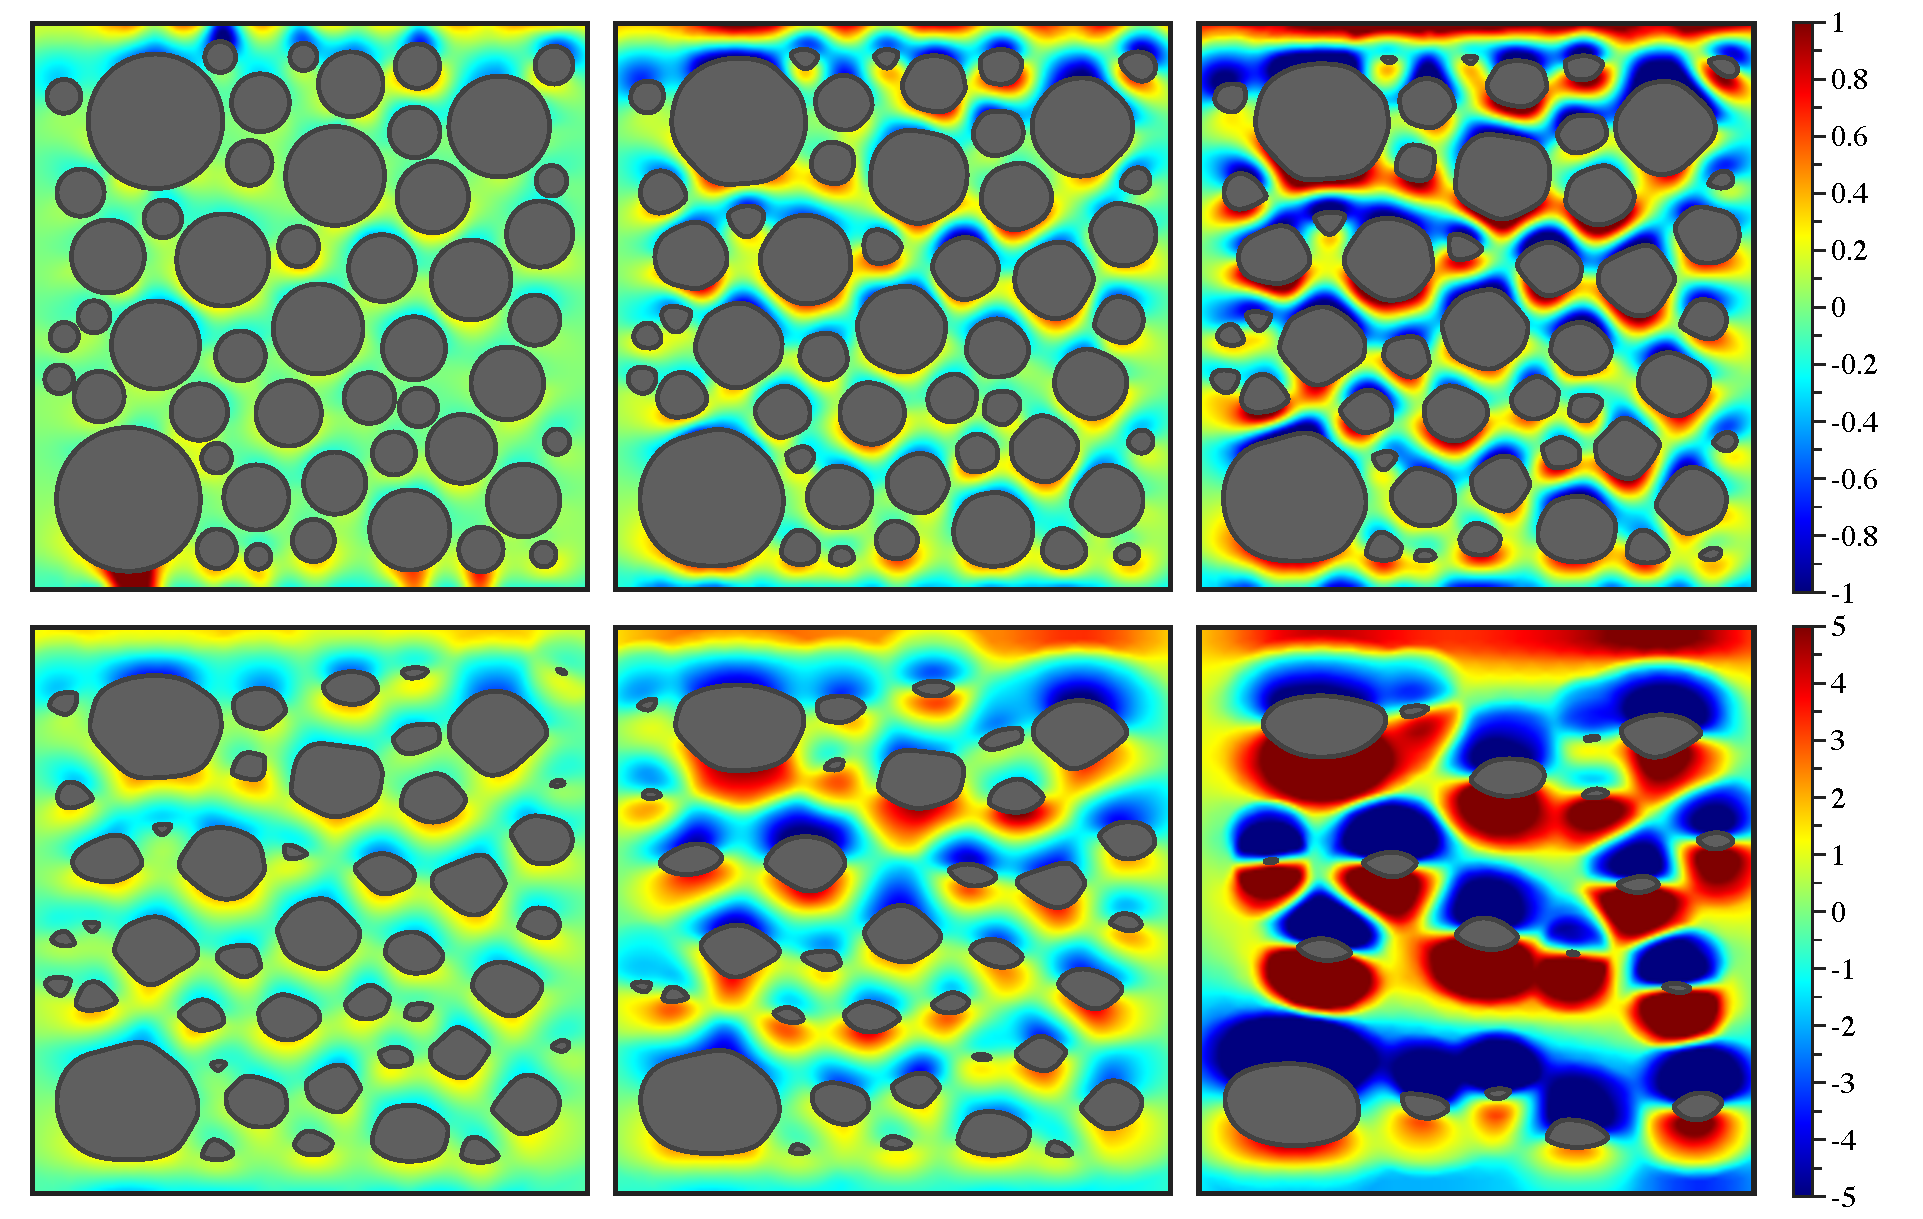
\includegraphics[width = 0.9 \textwidth]{./figs/50bod.pdf}
\caption{\label{fig:50bodies} A time lapse of 50 bodies eroding in a
viscous flow.  The boundary conditions are a constant pressure drop that
creates a flow from the left to right.  The rate of erosion is
proportional to the shear stress which is equivalent to the vorticity
evaluated on the bodies.  The colors represent the vorticity, so regions
with large vorticity (in magnitude) are regions where the flow will
erode the fastest.}
\end{center}
\end{figure}
 %^^^^^^^^^^^^^^^^^^^^^^^^^^^^^^%
% Figure generated from data file 50circ512p5, 
%which uses 50circ512.in with epsfac = 30, sigfac = 10, dt = 1e-4, fixpdrop = 1




%%%%%%%%%%%%%%%%%%%%%%%%%%%%%%%%%%%%%%%%%%%%%%%%%%%%%%%%%%%%%%%%%%%%%%%
\paragraph{Limitations} 

We begin by making two fundamental design choices: first, we restrict
ourselves to two spatial dimensions, and second the bodies are
considered immobile (i.e.~fixed to their initial locations). The
restriction to two dimensions allows us to simulate the erosion of many bodies
(up to $50$ in this manuscript) with high resolution, giving us the
ability to accurately characterize the erosion of a porous medium. While
BIEs are available in three dimensions, the extra computational cost limits the number of bodies that could be practically simulated, making porous-medium simulations less feasible. The second assumption of immobile bodies affords a simple framework to study the effects of erosion in isolation. While other effects, such as sedimentation or transport, undoubtedly play a role in real applications, these effects would introduce additional complexity, both conceptually and numerically. 


%%%%%%%%%%%%%%%%%%%%%%%%%%%%%%%%%%%%%%%%%%%%%%%%%%%%%%%%%%%%%%%%%%%%%%%
\paragraph{Related work} Simulating eroding bodies has been studied
analytically, experimentally, and numerically.  Many of these works are
motivated by high Reynolds number geophysical applications, such as the
work of the second author~\cite{moo-ris-chi-zha-she2013,
ris-moo-chi-she-zha2012, moore2017riemann} and others~\cite{par-izu2000,
lag2000, coh-dev-sey-yi-szy-rot2015, han1969, Rothman2012,
hewett2017evolution, ristroph2018sculpting, lopez2018cfd,
lachaussee2018competitive, cohen2016erosion}.  The work most closely
related to ours simulates erosion in a three-dimensional incompressible
Stokesian fluid~\cite{mit-spa2016}, but they only consider single
eroding body.  

The effect of erosion on a geometry is quite rich.  For instance, it has
been hypothesized and numerically observed that the erosion leads to a
shear stress that is uniform on the body which results in a uniform
erosion rate.  The shape that has a uniform shear stress is analyzed in
three dimensions by Montenegro-Johnson and Lauga~\cite{mon-lau2015}
which is an extension of the analysis done by Pironneau~\cite{pir1973}
to find a Stokesian drag minimizing shape.  In this idealized case,
analytical axisymmetric shapes that minimize the drag can be found.
However, the effect of erosion on a porous media is less understood.

To simulate multiple bodies, it is essential to resolve the nonlocal
effects between the different bodies.  In this work, these interactions
are included with high-order accuracy by using an integral equation
method.  Integral equations have been used extensively to simulate
viscous fluids in complex geometries.  One particular application are
particulate flows, such as bubbles or droplets, and the classic book of
Pozrikidis~\cite{poz1992} describes BIEs for such problems.  For nearly
touching bodies, the quadrature associated with discretizing a BIE can
lead to instabilities of specialized quadrature is not applied.  Since
our bodies do not move, we are able to use upsampling, but future work
will require a near-singular integration scheme~\cite{qua-bir2014a,
klo-bar-gre-one2013, bar-wu-vee2015, hel-oja2008a, bea-lai2001}.


%%%%%%%%%%%%%%%%%%%%%%%%%%%%%%%%%%%%%%%%%%%%%%%%%%%%%%%%%%%%%%%%%%%%%%%
\paragraph{Outline of the paper} In Section~\ref{s:formulation}, we
describe the governing equations for both the fluid and describe the
erosion model using a \thL~framework.  In Section~\ref{s:method}, the
numerical methods in both space and time are described and
Section~\ref{s:qoi} describes how to compute the vorticity, pressure,
and drag. Section~\ref{s:SingleResults} gives several numerical examples
for a single body, and Section~\ref{s:MultiResults} presents numerical
  examples for multiply-connected domains.  Finally, concluding remarks are made in Section~\ref{s:conclusions}




%%%%%%%%%%%%%%%%%%%%%%%%%%%%%%%%%%%%%%%%%%%%%%%%%%%%%%%%%%%%%%%%%%%%%%%
\section{Formulation}
\label{s:formulation}
We start by defining the main variables used to model erosion.  We
consider flows that are confined by a solid wall $\Gamma$ that encloses
$M$ eroding bodies as diagrammed in Fig.~\ref{fig:schematic}.  The
bodies are denoted as $\gamma_\ell$, $\ell=1,\ldots,M$, and we write
$\gamma = \gamma_1 \cup \cdots \cup \gamma_M$.  On each body, $\nn$ and
$\ss$ denote the unit normal and unit tangent vectors respectively.
Throughout the paper, we adopt the convention that $\ss$ points in the
counterclockwise direction and $\nn$ points out of the fluid domain
(i.e.~into the bodies). Neglecting inertial forces, the dynamics of the
fluid is fully determined by the position of the bodies $\xx_\ell(s,t)
\in \gamma_\ell$, where $s$ is the arclength and $t$ is time.  Given
$\xx_\ell(s,t)$, $\ell=1,\ldots,M$, derived variables include the fluid
velocity $\uu$, the pressure $p$, and the shear stress $\tau$.   On the
bounding wall, we prescribe a velocity $\UU(\xx,t)$.  Then, the
governing equations are
\begin{equation}
\label{eqn:erosionModel}
\begin{split}
  \mu \Delta \uu = \grad p, &\hspace{20pt} \xx \in \Omega, \gap &&\mbox{conservation
of momentum}\\
\grad \cdot \uu = 0, &\hspace{20pt} \xx \in \Omega, \gap
&&\mbox{\em conservation of mass} \\
\uu = 0, &\hspace{20pt} \xx \in \gamma, \gap &&\mbox{\em no slip on the
bodies} \\
\uu = \UU, &\hspace{20pt} \xx \in \Gamma, \gap &&\mbox{\em outer wall
velocity} \\
\Vn = \abs{\tau}, &\hspace{20pt} \xx \in \gamma,
&&\mbox{\em erosion model},
\end{split}
\end{equation}
where $\Vn$ is the normal velocity of the interface and $\mu$ is the
fluid viscosity.  There are several models for
erosion~\cite{par-izu2000,lag2000}, but we have adopted the model that
erosion occurs in the normal direction at a rate that is proportional to
the magnitude of the shear stress~\cite{moo-ris-chi-zha-she2013}.  The
constant of proportionality only sets the time scale, so we have set
$\Vn = |\tau|$ as described in equation~\eqref{eqn:erosionModel}.  For
the sake of numerical stability, we modify this law in
Section~\ref{sec:thetaL}. 

The outer wall is formed by rounding off the corners
of $[-3,3] \times [-1,1]$, and we impose the Hagen-Poiseuille flow
\begin{align*}
  \UU(\xx) = \umax (1-y^2,0), \quad \xx \in \Gamma,
\end{align*}
where $U$ sets the maximum of the imposed Poiseuille flow. Often, we
will simply set $U=1$, but in some instances we change $U$ dynamically
to enforce that the pressure drop across the computational cell is
constant as bodies erode within it.  The boundary of the fluid domain is
$\bd\Omega = \gamma_1 \cup \cdots \cup \gamma_M \cup \Gamma$.  To
minimize the boundary effects of the inflow and outflow, we only place
bodies in the center third, $[-1,1] \times [-1,1]$, of the fluid domain.

\begin{figure}[htpb]
  \centering
  \begin{tikzpicture}[scale=1.5] 

\begin{axis}[ 
axis equal image, 
scale only axis, 
xmin=-3.04, 
xmax=3.6, 
ymin=-1.1, 
ymax=1.1, 
hide axis, 
] 

\addplot [color=black,dashed,line width=1] coordinates{ 
  (-1,-1)
  (-1,+1)
}; 

\addplot [color=black,dashed,line width=1] coordinates{ 
  (1,-1)
  (1,+1)
}; 

\addplot [color=black,solid,line width=2] coordinates{ 
(3.0000e+00,0.0000e+00)
(3.0000e+00,2.4549e-02)
(3.0000e+00,4.9127e-02)
(3.0000e+00,7.3764e-02)
(3.0000e+00,9.8491e-02)
(3.0000e+00,1.2334e-01)
(3.0000e+00,1.4834e-01)
(3.0000e+00,1.7352e-01)
(3.0000e+00,1.9891e-01)
(3.0000e+00,2.2456e-01)
(3.0000e+00,2.5049e-01)
(3.0000e+00,2.7674e-01)
(3.0000e+00,3.0334e-01)
(2.9999e+00,3.3035e-01)
(2.9999e+00,3.5779e-01)
(2.9998e+00,3.8572e-01)
(2.9997e+00,4.1417e-01)
(2.9994e+00,4.4319e-01)
(2.9991e+00,4.7282e-01)
(2.9985e+00,5.0310e-01)
(2.9975e+00,5.3407e-01)
(2.9960e+00,5.6575e-01)
(2.9938e+00,5.9814e-01)
(2.9904e+00,6.3123e-01)
(2.9854e+00,6.6493e-01)
(2.9780e+00,6.9912e-01)
(2.9673e+00,7.3358e-01)
(2.9520e+00,7.6793e-01)
(2.9306e+00,8.0171e-01)
(2.9014e+00,8.3425e-01)
(2.8625e+00,8.6481e-01)
(2.8126e+00,8.9262e-01)
(2.7510e+00,9.1700e-01)
(2.6779e+00,9.3755e-01)
(2.5944e+00,9.5418e-01)
(2.5028e+00,9.6713e-01)
(2.4051e+00,9.7688e-01)
(2.3038e+00,9.8402e-01)
(2.2007e+00,9.8911e-01)
(2.0974e+00,9.9268e-01)
(1.9948e+00,9.9514e-01)
(1.8937e+00,9.9681e-01)
(1.7944e+00,9.9794e-01)
(1.6972e+00,9.9868e-01)
(1.6022e+00,9.9917e-01)
(1.5093e+00,9.9949e-01)
(1.4185e+00,9.9969e-01)
(1.3296e+00,9.9981e-01)
(1.2425e+00,9.9989e-01)
(1.1572e+00,9.9994e-01)
(1.0734e+00,9.9997e-01)
(9.9105e-01,9.9998e-01)
(9.1003e-01,9.9999e-01)
(8.3021e-01,1.0000e+00)
(7.5146e-01,1.0000e+00)
(6.7367e-01,1.0000e+00)
(5.9674e-01,1.0000e+00)
(5.2055e-01,1.0000e+00)
(4.4501e-01,1.0000e+00)
(3.7001e-01,1.0000e+00)
(2.9547e-01,1.0000e+00)
(2.2129e-01,1.0000e+00)
(1.4738e-01,1.0000e+00)
(7.3646e-02,1.0000e+00)
(1.8370e-16,1.0000e+00)
(-7.3646e-02,1.0000e+00)
(-1.4738e-01,1.0000e+00)
(-2.2129e-01,1.0000e+00)
(-2.9547e-01,1.0000e+00)
(-3.7001e-01,1.0000e+00)
(-4.4501e-01,1.0000e+00)
(-5.2055e-01,1.0000e+00)
(-5.9674e-01,1.0000e+00)
(-6.7367e-01,1.0000e+00)
(-7.5146e-01,1.0000e+00)
(-8.3021e-01,1.0000e+00)
(-9.1003e-01,9.9999e-01)
(-9.9105e-01,9.9998e-01)
(-1.0734e+00,9.9997e-01)
(-1.1572e+00,9.9994e-01)
(-1.2425e+00,9.9989e-01)
(-1.3296e+00,9.9981e-01)
(-1.4185e+00,9.9969e-01)
(-1.5093e+00,9.9949e-01)
(-1.6022e+00,9.9917e-01)
(-1.6972e+00,9.9868e-01)
(-1.7944e+00,9.9794e-01)
(-1.8937e+00,9.9681e-01)
(-1.9948e+00,9.9514e-01)
(-2.0974e+00,9.9268e-01)
(-2.2007e+00,9.8911e-01)
(-2.3038e+00,9.8402e-01)
(-2.4051e+00,9.7688e-01)
(-2.5028e+00,9.6713e-01)
(-2.5944e+00,9.5418e-01)
(-2.6779e+00,9.3755e-01)
(-2.7510e+00,9.1700e-01)
(-2.8126e+00,8.9262e-01)
(-2.8625e+00,8.6481e-01)
(-2.9014e+00,8.3425e-01)
(-2.9306e+00,8.0171e-01)
(-2.9520e+00,7.6793e-01)
(-2.9673e+00,7.3358e-01)
(-2.9780e+00,6.9912e-01)
(-2.9854e+00,6.6493e-01)
(-2.9904e+00,6.3123e-01)
(-2.9938e+00,5.9814e-01)
(-2.9960e+00,5.6575e-01)
(-2.9975e+00,5.3407e-01)
(-2.9985e+00,5.0310e-01)
(-2.9991e+00,4.7282e-01)
(-2.9994e+00,4.4319e-01)
(-2.9997e+00,4.1417e-01)
(-2.9998e+00,3.8572e-01)
(-2.9999e+00,3.5779e-01)
(-2.9999e+00,3.3035e-01)
(-3.0000e+00,3.0334e-01)
(-3.0000e+00,2.7674e-01)
(-3.0000e+00,2.5049e-01)
(-3.0000e+00,2.2456e-01)
(-3.0000e+00,1.9891e-01)
(-3.0000e+00,1.7352e-01)
(-3.0000e+00,1.4834e-01)
(-3.0000e+00,1.2334e-01)
(-3.0000e+00,9.8491e-02)
(-3.0000e+00,7.3764e-02)
(-3.0000e+00,4.9127e-02)
(-3.0000e+00,2.4549e-02)
(-3.0000e+00,1.2246e-16)
(-3.0000e+00,-2.4549e-02)
(-3.0000e+00,-4.9127e-02)
(-3.0000e+00,-7.3764e-02)
(-3.0000e+00,-9.8491e-02)
(-3.0000e+00,-1.2334e-01)
(-3.0000e+00,-1.4834e-01)
(-3.0000e+00,-1.7352e-01)
(-3.0000e+00,-1.9891e-01)
(-3.0000e+00,-2.2456e-01)
(-3.0000e+00,-2.5049e-01)
(-3.0000e+00,-2.7674e-01)
(-3.0000e+00,-3.0334e-01)
(-2.9999e+00,-3.3035e-01)
(-2.9999e+00,-3.5779e-01)
(-2.9998e+00,-3.8572e-01)
(-2.9997e+00,-4.1417e-01)
(-2.9994e+00,-4.4319e-01)
(-2.9991e+00,-4.7282e-01)
(-2.9985e+00,-5.0310e-01)
(-2.9975e+00,-5.3407e-01)
(-2.9960e+00,-5.6575e-01)
(-2.9938e+00,-5.9814e-01)
(-2.9904e+00,-6.3123e-01)
(-2.9854e+00,-6.6493e-01)
(-2.9780e+00,-6.9912e-01)
(-2.9673e+00,-7.3358e-01)
(-2.9520e+00,-7.6793e-01)
(-2.9306e+00,-8.0171e-01)
(-2.9014e+00,-8.3425e-01)
(-2.8625e+00,-8.6481e-01)
(-2.8126e+00,-8.9262e-01)
(-2.7510e+00,-9.1700e-01)
(-2.6779e+00,-9.3755e-01)
(-2.5944e+00,-9.5418e-01)
(-2.5028e+00,-9.6713e-01)
(-2.4051e+00,-9.7688e-01)
(-2.3038e+00,-9.8402e-01)
(-2.2007e+00,-9.8911e-01)
(-2.0974e+00,-9.9268e-01)
(-1.9948e+00,-9.9514e-01)
(-1.8937e+00,-9.9681e-01)
(-1.7944e+00,-9.9794e-01)
(-1.6972e+00,-9.9868e-01)
(-1.6022e+00,-9.9917e-01)
(-1.5093e+00,-9.9949e-01)
(-1.4185e+00,-9.9969e-01)
(-1.3296e+00,-9.9981e-01)
(-1.2425e+00,-9.9989e-01)
(-1.1572e+00,-9.9994e-01)
(-1.0734e+00,-9.9997e-01)
(-9.9105e-01,-9.9998e-01)
(-9.1003e-01,-9.9999e-01)
(-8.3021e-01,-1.0000e+00)
(-7.5146e-01,-1.0000e+00)
(-6.7367e-01,-1.0000e+00)
(-5.9674e-01,-1.0000e+00)
(-5.2055e-01,-1.0000e+00)
(-4.4501e-01,-1.0000e+00)
(-3.7001e-01,-1.0000e+00)
(-2.9547e-01,-1.0000e+00)
(-2.2129e-01,-1.0000e+00)
(-1.4738e-01,-1.0000e+00)
(-7.3646e-02,-1.0000e+00)
(-5.5109e-16,-1.0000e+00)
(7.3646e-02,-1.0000e+00)
(1.4738e-01,-1.0000e+00)
(2.2129e-01,-1.0000e+00)
(2.9547e-01,-1.0000e+00)
(3.7001e-01,-1.0000e+00)
(4.4501e-01,-1.0000e+00)
(5.2055e-01,-1.0000e+00)
(5.9674e-01,-1.0000e+00)
(6.7367e-01,-1.0000e+00)
(7.5146e-01,-1.0000e+00)
(8.3021e-01,-1.0000e+00)
(9.1003e-01,-9.9999e-01)
(9.9105e-01,-9.9998e-01)
(1.0734e+00,-9.9997e-01)
(1.1572e+00,-9.9994e-01)
(1.2425e+00,-9.9989e-01)
(1.3296e+00,-9.9981e-01)
(1.4185e+00,-9.9969e-01)
(1.5093e+00,-9.9949e-01)
(1.6022e+00,-9.9917e-01)
(1.6972e+00,-9.9868e-01)
(1.7944e+00,-9.9794e-01)
(1.8937e+00,-9.9681e-01)
(1.9948e+00,-9.9514e-01)
(2.0974e+00,-9.9268e-01)
(2.2007e+00,-9.8911e-01)
(2.3038e+00,-9.8402e-01)
(2.4051e+00,-9.7688e-01)
(2.5028e+00,-9.6713e-01)
(2.5944e+00,-9.5418e-01)
(2.6779e+00,-9.3755e-01)
(2.7510e+00,-9.1700e-01)
(2.8126e+00,-8.9262e-01)
(2.8625e+00,-8.6481e-01)
(2.9014e+00,-8.3425e-01)
(2.9306e+00,-8.0171e-01)
(2.9520e+00,-7.6793e-01)
(2.9673e+00,-7.3358e-01)
(2.9780e+00,-6.9912e-01)
(2.9854e+00,-6.6493e-01)
(2.9904e+00,-6.3123e-01)
(2.9938e+00,-5.9814e-01)
(2.9960e+00,-5.6575e-01)
(2.9975e+00,-5.3407e-01)
(2.9985e+00,-5.0310e-01)
(2.9991e+00,-4.7282e-01)
(2.9994e+00,-4.4319e-01)
(2.9997e+00,-4.1417e-01)
(2.9998e+00,-3.8572e-01)
(2.9999e+00,-3.5779e-01)
(2.9999e+00,-3.3035e-01)
(3.0000e+00,-3.0334e-01)
(3.0000e+00,-2.7674e-01)
(3.0000e+00,-2.5049e-01)
(3.0000e+00,-2.2456e-01)
(3.0000e+00,-1.9891e-01)
(3.0000e+00,-1.7352e-01)
(3.0000e+00,-1.4834e-01)
(3.0000e+00,-1.2334e-01)
(3.0000e+00,-9.8491e-02)
(3.0000e+00,-7.3764e-02)
(3.0000e+00,-4.9127e-02)
(3.0000e+00,-2.4549e-02)
(3.0000e+00,0.0000e+00)
}; 

\addplot [color=black,solid,fill] coordinates{ 
(5.0000e-01,0.0000e+00)
(4.9759e-01,4.9009e-02)
(4.9039e-01,9.7545e-02)
(4.7847e-01,1.4514e-01)
(4.6194e-01,1.9134e-01)
(4.4096e-01,2.3570e-01)
(4.1573e-01,2.7779e-01)
(3.8651e-01,3.1720e-01)
(3.5355e-01,3.5355e-01)
(3.1720e-01,3.8651e-01)
(2.7779e-01,4.1573e-01)
(2.3570e-01,4.4096e-01)
(1.9134e-01,4.6194e-01)
(1.4514e-01,4.7847e-01)
(9.7545e-02,4.9039e-01)
(4.9009e-02,4.9759e-01)
(3.0616e-17,5.0000e-01)
(-4.9009e-02,4.9759e-01)
(-9.7545e-02,4.9039e-01)
(-1.4514e-01,4.7847e-01)
(-1.9134e-01,4.6194e-01)
(-2.3570e-01,4.4096e-01)
(-2.7779e-01,4.1573e-01)
(-3.1720e-01,3.8651e-01)
(-3.5355e-01,3.5355e-01)
(-3.8651e-01,3.1720e-01)
(-4.1573e-01,2.7779e-01)
(-4.4096e-01,2.3570e-01)
(-4.6194e-01,1.9134e-01)
(-4.7847e-01,1.4514e-01)
(-4.9039e-01,9.7545e-02)
(-4.9759e-01,4.9009e-02)
(-5.0000e-01,6.1232e-17)
(-4.9759e-01,-4.9009e-02)
(-4.9039e-01,-9.7545e-02)
(-4.7847e-01,-1.4514e-01)
(-4.6194e-01,-1.9134e-01)
(-4.4096e-01,-2.3570e-01)
(-4.1573e-01,-2.7779e-01)
(-3.8651e-01,-3.1720e-01)
(-3.5355e-01,-3.5355e-01)
(-3.1720e-01,-3.8651e-01)
(-2.7779e-01,-4.1573e-01)
(-2.3570e-01,-4.4096e-01)
(-1.9134e-01,-4.6194e-01)
(-1.4514e-01,-4.7847e-01)
(-9.7545e-02,-4.9039e-01)
(-4.9009e-02,-4.9759e-01)
(-9.1849e-17,-5.0000e-01)
(4.9009e-02,-4.9759e-01)
(9.7545e-02,-4.9039e-01)
(1.4514e-01,-4.7847e-01)
(1.9134e-01,-4.6194e-01)
(2.3570e-01,-4.4096e-01)
(2.7779e-01,-4.1573e-01)
(3.1720e-01,-3.8651e-01)
(3.5355e-01,-3.5355e-01)
(3.8651e-01,-3.1720e-01)
(4.1573e-01,-2.7779e-01)
(4.4096e-01,-2.3570e-01)
(4.6194e-01,-1.9134e-01)
(4.7847e-01,-1.4514e-01)
(4.9039e-01,-9.7545e-02)
(4.9759e-01,-4.9009e-02)
(5.0000e-01,-1.2246e-16)
};

\addplot [color=black,solid,fill] coordinates{ 
(8.0000e-01,5.0000e-01)
(7.9952e-01,5.0980e-01)
(7.9808e-01,5.1951e-01)
(7.9569e-01,5.2903e-01)
(7.9239e-01,5.3827e-01)
(7.8819e-01,5.4714e-01)
(7.8315e-01,5.5556e-01)
(7.7730e-01,5.6344e-01)
(7.7071e-01,5.7071e-01)
(7.6344e-01,5.7730e-01)
(7.5556e-01,5.8315e-01)
(7.4714e-01,5.8819e-01)
(7.3827e-01,5.9239e-01)
(7.2903e-01,5.9569e-01)
(7.1951e-01,5.9808e-01)
(7.0980e-01,5.9952e-01)
(7.0000e-01,6.0000e-01)
(6.9020e-01,5.9952e-01)
(6.8049e-01,5.9808e-01)
(6.7097e-01,5.9569e-01)
(6.6173e-01,5.9239e-01)
(6.5286e-01,5.8819e-01)
(6.4444e-01,5.8315e-01)
(6.3656e-01,5.7730e-01)
(6.2929e-01,5.7071e-01)
(6.2270e-01,5.6344e-01)
(6.1685e-01,5.5556e-01)
(6.1181e-01,5.4714e-01)
(6.0761e-01,5.3827e-01)
(6.0431e-01,5.2903e-01)
(6.0192e-01,5.1951e-01)
(6.0048e-01,5.0980e-01)
(6.0000e-01,5.0000e-01)
(6.0048e-01,4.9020e-01)
(6.0192e-01,4.8049e-01)
(6.0431e-01,4.7097e-01)
(6.0761e-01,4.6173e-01)
(6.1181e-01,4.5286e-01)
(6.1685e-01,4.4444e-01)
(6.2270e-01,4.3656e-01)
(6.2929e-01,4.2929e-01)
(6.3656e-01,4.2270e-01)
(6.4444e-01,4.1685e-01)
(6.5286e-01,4.1181e-01)
(6.6173e-01,4.0761e-01)
(6.7097e-01,4.0431e-01)
(6.8049e-01,4.0192e-01)
(6.9020e-01,4.0048e-01)
(7.0000e-01,4.0000e-01)
(7.0980e-01,4.0048e-01)
(7.1951e-01,4.0192e-01)
(7.2903e-01,4.0431e-01)
(7.3827e-01,4.0761e-01)
(7.4714e-01,4.1181e-01)
(7.5556e-01,4.1685e-01)
(7.6344e-01,4.2270e-01)
(7.7071e-01,4.2929e-01)
(7.7730e-01,4.3656e-01)
(7.8315e-01,4.4444e-01)
(7.8819e-01,4.5286e-01)
(7.9239e-01,4.6173e-01)
(7.9569e-01,4.7097e-01)
(7.9808e-01,4.8049e-01)
(7.9952e-01,4.9020e-01)
(8.0000e-01,5.0000e-01)
};

\addplot [color=black,solid,fill] coordinates{ 
(-6.0000e-01,6.0000e-01)
(-6.0096e-01,6.1960e-01)
(-6.0384e-01,6.3902e-01)
(-6.0861e-01,6.5806e-01)
(-6.1522e-01,6.7654e-01)
(-6.2362e-01,6.9428e-01)
(-6.3371e-01,7.1111e-01)
(-6.4540e-01,7.2688e-01)
(-6.5858e-01,7.4142e-01)
(-6.7312e-01,7.5460e-01)
(-6.8889e-01,7.6629e-01)
(-7.0572e-01,7.7638e-01)
(-7.2346e-01,7.8478e-01)
(-7.4194e-01,7.9139e-01)
(-7.6098e-01,7.9616e-01)
(-7.8040e-01,7.9904e-01)
(-8.0000e-01,8.0000e-01)
(-8.1960e-01,7.9904e-01)
(-8.3902e-01,7.9616e-01)
(-8.5806e-01,7.9139e-01)
(-8.7654e-01,7.8478e-01)
(-8.9428e-01,7.7638e-01)
(-9.1111e-01,7.6629e-01)
(-9.2688e-01,7.5460e-01)
(-9.4142e-01,7.4142e-01)
(-9.5460e-01,7.2688e-01)
(-9.6629e-01,7.1111e-01)
(-9.7638e-01,6.9428e-01)
(-9.8478e-01,6.7654e-01)
(-9.9139e-01,6.5806e-01)
(-9.9616e-01,6.3902e-01)
(-9.9904e-01,6.1960e-01)
(-1.0000e+00,6.0000e-01)
(-9.9904e-01,5.8040e-01)
(-9.9616e-01,5.6098e-01)
(-9.9139e-01,5.4194e-01)
(-9.8478e-01,5.2346e-01)
(-9.7638e-01,5.0572e-01)
(-9.6629e-01,4.8889e-01)
(-9.5460e-01,4.7312e-01)
(-9.4142e-01,4.5858e-01)
(-9.2688e-01,4.4540e-01)
(-9.1111e-01,4.3371e-01)
(-8.9428e-01,4.2362e-01)
(-8.7654e-01,4.1522e-01)
(-8.5806e-01,4.0861e-01)
(-8.3902e-01,4.0384e-01)
(-8.1960e-01,4.0096e-01)
(-8.0000e-01,4.0000e-01)
(-7.8040e-01,4.0096e-01)
(-7.6098e-01,4.0384e-01)
(-7.4194e-01,4.0861e-01)
(-7.2346e-01,4.1522e-01)
(-7.0572e-01,4.2362e-01)
(-6.8889e-01,4.3371e-01)
(-6.7312e-01,4.4540e-01)
(-6.5858e-01,4.5858e-01)
(-6.4540e-01,4.7312e-01)
(-6.3371e-01,4.8889e-01)
(-6.2362e-01,5.0572e-01)
(-6.1522e-01,5.2346e-01)
(-6.0861e-01,5.4194e-01)
(-6.0384e-01,5.6098e-01)
(-6.0096e-01,5.8040e-01)
(-6.0000e-01,6.0000e-01)
};

\addplot [color=black,solid,fill] coordinates{ 
(9.0000e-01,-6.0000e-01)
(8.9904e-01,-5.8040e-01)
(8.9616e-01,-5.6098e-01)
(8.9139e-01,-5.4194e-01)
(8.8478e-01,-5.2346e-01)
(8.7638e-01,-5.0572e-01)
(8.6629e-01,-4.8889e-01)
(8.5460e-01,-4.7312e-01)
(8.4142e-01,-4.5858e-01)
(8.2688e-01,-4.4540e-01)
(8.1111e-01,-4.3371e-01)
(7.9428e-01,-4.2362e-01)
(7.7654e-01,-4.1522e-01)
(7.5806e-01,-4.0861e-01)
(7.3902e-01,-4.0384e-01)
(7.1960e-01,-4.0096e-01)
(7.0000e-01,-4.0000e-01)
(6.8040e-01,-4.0096e-01)
(6.6098e-01,-4.0384e-01)
(6.4194e-01,-4.0861e-01)
(6.2346e-01,-4.1522e-01)
(6.0572e-01,-4.2362e-01)
(5.8889e-01,-4.3371e-01)
(5.7312e-01,-4.4540e-01)
(5.5858e-01,-4.5858e-01)
(5.4540e-01,-4.7312e-01)
(5.3371e-01,-4.8889e-01)
(5.2362e-01,-5.0572e-01)
(5.1522e-01,-5.2346e-01)
(5.0861e-01,-5.4194e-01)
(5.0384e-01,-5.6098e-01)
(5.0096e-01,-5.8040e-01)
(5.0000e-01,-6.0000e-01)
(5.0096e-01,-6.1960e-01)
(5.0384e-01,-6.3902e-01)
(5.0861e-01,-6.5806e-01)
(5.1522e-01,-6.7654e-01)
(5.2362e-01,-6.9428e-01)
(5.3371e-01,-7.1111e-01)
(5.4540e-01,-7.2688e-01)
(5.5858e-01,-7.4142e-01)
(5.7312e-01,-7.5460e-01)
(5.8889e-01,-7.6629e-01)
(6.0572e-01,-7.7638e-01)
(6.2346e-01,-7.8478e-01)
(6.4194e-01,-7.9139e-01)
(6.6098e-01,-7.9616e-01)
(6.8040e-01,-7.9904e-01)
(7.0000e-01,-8.0000e-01)
(7.1960e-01,-7.9904e-01)
(7.3902e-01,-7.9616e-01)
(7.5806e-01,-7.9139e-01)
(7.7654e-01,-7.8478e-01)
(7.9428e-01,-7.7638e-01)
(8.1111e-01,-7.6629e-01)
(8.2688e-01,-7.5460e-01)
(8.4142e-01,-7.4142e-01)
(8.5460e-01,-7.2688e-01)
(8.6629e-01,-7.1111e-01)
(8.7638e-01,-6.9428e-01)
(8.8478e-01,-6.7654e-01)
(8.9139e-01,-6.5806e-01)
(8.9616e-01,-6.3902e-01)
(8.9904e-01,-6.1960e-01)
(9.0000e-01,-6.0000e-01)
};

\addplot [color=black,solid,fill] coordinates{ 
(-6.4000e-01,-5.0000e-01)
(-6.4029e-01,-4.9412e-01)
(-6.4115e-01,-4.8829e-01)
(-6.4258e-01,-4.8258e-01)
(-6.4457e-01,-4.7704e-01)
(-6.4708e-01,-4.7172e-01)
(-6.5011e-01,-4.6667e-01)
(-6.5362e-01,-4.6194e-01)
(-6.5757e-01,-4.5757e-01)
(-6.6194e-01,-4.5362e-01)
(-6.6667e-01,-4.5011e-01)
(-6.7172e-01,-4.4708e-01)
(-6.7704e-01,-4.4457e-01)
(-6.8258e-01,-4.4258e-01)
(-6.8829e-01,-4.4115e-01)
(-6.9412e-01,-4.4029e-01)
(-7.0000e-01,-4.4000e-01)
(-7.0588e-01,-4.4029e-01)
(-7.1171e-01,-4.4115e-01)
(-7.1742e-01,-4.4258e-01)
(-7.2296e-01,-4.4457e-01)
(-7.2828e-01,-4.4708e-01)
(-7.3333e-01,-4.5011e-01)
(-7.3806e-01,-4.5362e-01)
(-7.4243e-01,-4.5757e-01)
(-7.4638e-01,-4.6194e-01)
(-7.4989e-01,-4.6667e-01)
(-7.5292e-01,-4.7172e-01)
(-7.5543e-01,-4.7704e-01)
(-7.5742e-01,-4.8258e-01)
(-7.5885e-01,-4.8829e-01)
(-7.5971e-01,-4.9412e-01)
(-7.6000e-01,-5.0000e-01)
(-7.5971e-01,-5.0588e-01)
(-7.5885e-01,-5.1171e-01)
(-7.5742e-01,-5.1742e-01)
(-7.5543e-01,-5.2296e-01)
(-7.5292e-01,-5.2828e-01)
(-7.4989e-01,-5.3333e-01)
(-7.4638e-01,-5.3806e-01)
(-7.4243e-01,-5.4243e-01)
(-7.3806e-01,-5.4638e-01)
(-7.3333e-01,-5.4989e-01)
(-7.2828e-01,-5.5292e-01)
(-7.2296e-01,-5.5543e-01)
(-7.1742e-01,-5.5742e-01)
(-7.1171e-01,-5.5885e-01)
(-7.0588e-01,-5.5971e-01)
(-7.0000e-01,-5.6000e-01)
(-6.9412e-01,-5.5971e-01)
(-6.8829e-01,-5.5885e-01)
(-6.8258e-01,-5.5742e-01)
(-6.7704e-01,-5.5543e-01)
(-6.7172e-01,-5.5292e-01)
(-6.6667e-01,-5.4989e-01)
(-6.6194e-01,-5.4638e-01)
(-6.5757e-01,-5.4243e-01)
(-6.5362e-01,-5.3806e-01)
(-6.5011e-01,-5.3333e-01)
(-6.4708e-01,-5.2828e-01)
(-6.4457e-01,-5.2296e-01)
(-6.4258e-01,-5.1742e-01)
(-6.4115e-01,-5.1171e-01)
(-6.4029e-01,-5.0588e-01)
(-6.4000e-01,-5.0000e-01)
};

%\draw[step=50] (0,0) grid (1200,300);

\node[font = \Huge,color=black] at (500,110) {$\Omega$};
\node[font = \normalsize,color=red] at (338,122) {$\nn$};
\node[font = \normalsize,color=red] at (342,158) {$\ss$};
\path[->,line width=1.2](240,90) edge (260,100);
\node at (225,90) {$\gamma_k$};
\path[->,line width=1.2,color=black](140,50) edge (120,14);
\node[font = \Large,color=black] at (150,70) {$\Gamma$};

\foreach \y in {-0.7,-0.5,...,0.7}
\addplot[color=black,line width = 1.0pt,solid,->]
plot coordinates{
  (-3,\y)
  (-3+0.6*(1-\y*\y),\y)
};

\foreach \y in {-0.7,-0.5,...,0.7}
\addplot[color=black,line width = 1.0pt,solid,->]
plot coordinates{
  (3,\y)
  (3+0.6*(1-\y*\y),\y)
};

\addplot[color=red,line width=0.5pt,solid,->]
plot coordinates{
  (0.3865,0.3172)
  (0.0966,0.0793)
};

\addplot[color=red,line width=0.5pt,solid,->]
plot coordinates{
  (0.3865,0.3172)
  (0.1486,0.6071)
};


\end{axis}

\end{tikzpicture}


  \caption{\label{fig:schematic} A schematic for the governing
    equations.  A no-slip boundary condition is imposed on each body
    $\gamma_\ell$ whose unit normal points outward relative to the
    geometry.  On the outer geometry $\Gamma$, a Hagen-Poiseuille flow
    is imposed.  The bodies are eroded at a rate that is proportional to
    the magnitude of the shear stress applied by the Stokesian fluid.
    The bodies are constrained to the middle third of the channel that
    is located between the dashed lines.}
\end{figure}

We describe how the incompressible Stokes equations are solved in
$\Omega$ using a boundary integral equation in Section~\ref{sec:bies}.
In Section~\ref{sec:shearStressLP}, we discuss how the shear stress is
computed.  Finally, in Section~\ref{sec:thetaL}, we describe how corners
in the geometry are avoided and perform a change of coordinates to treat
a stiff term.


%%%%%%%%%%%%%%%%%%%%%%%%%%%%%%%%%%%%%%%%%%%%%%%%%%%%%%%%%%%%%%%%%%%%%%%
\subsection{Boundary integral equation formulation} 
\label{sec:bies}

In this section, we describe an equivalent BIE formulation of the
incompressible Stokes equations with Dirichlet boundary conditions
\begin{equation}
  \begin{split}
  \mu\Delta \uu &= \grad p, \qquad && \xx \in \Omega, \\
  \grad \cdot \uu &= 0,   && \xx \in \Omega, \\
  \uu &= \ff,  && \xx \in \bd\Omega.
  \end{split}
  \label{eqn:stokes}
\end{equation}
The boundary condition $\ff$ is the prescribed velocity $\UU$ on
$\Gamma$, and it is zero on the eroding grains $\gamma$.  In two
dimensions, a BIE for a stream function formulation is
possible~\cite{gre-kro-may1996}, but this does not extend to three
dimensions.  Therefore, we adopt a primitive variable formulation where
the velocity is written in terms of the standard double-layer
potential~\cite{lad1963,poz1992}
\begin{align}
  \DD[\eeta](\xx) = \frac{1}{\pi} \int_{\bd\Omega} 
    \frac{\rr \cdot \nn}{\rho^2} \frac{\rr \otimes \rr}{\rho^2} 
    \eeta(\yy) \, ds_\yy, \quad \xx \in \Omega,
    \label{eqn:velocityDLP}
\end{align}
where $\rr = \xx - \yy$, $\rho = \|\rr\|$, and $\eeta$ is an unknown
density function.  As the viscosity $\mu$ also sets the time scale, we
take $\mu=1$.  \todo[inline]{Do you think we should flesh out this
time-scale stuff more precisely? i.e.~By setting $\mu = 1$ and $C = 1$
(the erosion constant), what exactly is the timescale that defines our
dimensionless time.} \todo[inline]{This might be worth doing.  Is it
something you can do quickly or do you want me to take a crack at it?}

Since the double-layer potential is not able to represent force- and
torque-free velocity fields,  we complete the double-layer potential
with Stokeslets and rotlets~\cite{pow-mir1987, pow1993}
\begin{align}
  S[\llambda_\ell,\cc_\ell] = \frac{1}{4\pi} \left(-\log \rho \II + 
    \frac{\rr \otimes \rr}{\rho^2} \right)\llambda_\ell
  \quad \text{and} \quad
  R[\xi_\ell,\cc_\ell] = \frac{\rr^\perp}{\rho^2}\xi_\ell, 
  \quad \ell=1,\ldots,M,
  \label{eqn:stokeslet_rotlet}
\end{align}
where  $\rr = \xx - \cc_\ell$, $\cc_\ell$ is a point inside the
$\ell^{th}$ grainy, $\rr^\perp = (r_2,-r_1)$, and $\rho = \|\rr\|$.
Then, the solution of~\eqref{eqn:stokes} is
\begin{align}
  \label{eqn:completed_DLP}
  \uu(\xx) = \DD[\eeta](\xx) + 
    \sum_{\ell=1}^{M} S[\llambda_\ell,\cc_\ell](\xx) +
    \sum_{\ell=1}^{M} R[\xi_\ell,\cc_\ell](\xx), \quad \xx \in \Omega,
\end{align}
where the density function, Stokeslets, and rotlets satisfy
\begin{subequations}
\label{eqn:completed_BIE}
\begin{align}
  \ff(\xx) &= -\frac{1}{2}\eeta(\xx) + \DD[\eeta](\xx) + 
      \sum_{\ell=1}^{M} S[\llambda_\ell,\cc_\ell](\xx) +
      \sum_{\ell=1}^{M} R[\xi_\ell,\cc_\ell](\xx) + \NN_0[\eeta](\xx),
      \quad \xx \in \bd\Omega, 
      \label{eqn:DLP}\\
  \llambda_\ell &= \frac{1}{2\pi}\int_{\gamma_\ell} \eeta(\yy) \, ds_\yy,
  \quad \ell=1,\ldots,M,
  \label{eqn:stokeslet} \\
  \xi_\ell &= \frac{1}{2\pi}\int_{\gamma_\ell} \yy^\perp \cdot \eeta(\yy)
  \, ds_\yy, \quad \ell=1,\ldots,M.
  \label{eqn:rotlet}
\end{align}
\end{subequations}
Here,
\begin{align*}
  \NN_0[\eeta](\xx) = \int_{\Gamma} 
    (\nn(\xx) \otimes \nn(\yy))\eeta(\yy) \, ds_\yy
\end{align*}
removes the rank one null space resulting from the flux-free requirement
of $\ff$.

This BIE formulation requires that $\bd\Omega$ is smooth.
Unfortunately, smoothness is not guaranteed erosion since corners
develop at locations where the shear stress vanishes.  One option is to
modify our BIE to handle corners~\cite{rac-ser2017,
ser-rok2016, hel2011, gil-hao-mar2014, bre2012}, but these methods
require the corner's location, or a non-uniform spaced mesh, or are
ill-conditioned.  Instead, make a slight modification to the erosion
model in Section~\ref{sec:thetaL} which allows us to control the
smoothness of the grains.  In this manner, the BIE as described above
can be applied.

%%%%%%%%%%%%%%%%%%%%%%%%%%%%%%%%%%%%%%%%%%%%%%%%%%%%%%%%%%%%%%%%%%%%%%%
\subsection{Computing the shear stress}
\label{sec:shearStressLP}
Once the density function, Stokeslets, and rotlets are computed, any
desired quantity, including the shear stress, can be computed.  The
shear stress is
\begin{align*}
  \tau = -\left(\nabla \uu + \nabla \uu^T \right)\nn \cdot \ss \, .
\end{align*}
The reader may notice an unusual sign convention above, but this is
simply a consequence of our conventions for $\nn$ and $\ss$ (see
Fig.~\ref{fig:schematic}).  The velocity field of the completed
double-layer potential~\eqref{eqn:completed_DLP} includes velocities
from three terms: the double-layer potential, the Stokeslets, and the
rotlets.  We compute the deformation tensor $\ssigma =
\frac{1}{2}(\nabla\uu + \nabla\uu^T)$ of these terms individually.

The deformation tensor of the double-layer
potential~\eqref{eqn:velocityDLP} at an interior point $\xx \in \Omega$
is~\cite{qua-bir2014a}
\begin{equation}
  \label{eqn:shearStressDLP}
  \begin{aligned}
  \ssigma^\DD(\xx) = \frac{1}{2\pi}\int_{\bd\Omega} &\left(
    2\frac{\rr \cdot \nn}{\rho^2} \frac{\rr \cdot \eeta}{\rho^2} \II + 
    \frac{\rr \cdot \eeta}{\rho^4} (\nn \otimes \rr + \rr \otimes \nn) 
    \right. \\
    &\left.
    +\frac{\rr \cdot \nn}{\rho^4} (\eeta \otimes \rr + \rr \otimes \eeta) - 
    8\frac{(\rr \cdot \nn)(\rr \cdot \eeta)}{\rho^6}(\rr \otimes \rr)
  \right) \eeta(\yy) ds_\yy.
  \end{aligned}
\end{equation}
We require the deformation tensor on $\bd\Omega$, and this requires
taking the limit of equation~\eqref{eqn:shearStressDLP} when $\xx$ tends
to $\xx_0 \in \bd\Omega$.  The limiting value is
\begin{align*}
  \lim_{\substack{\xx \rightarrow \xx_0 \\ \xx \in \Omega}}\sigma_\DD(\xx) =
  J[\eeta](\xx_0) + \ssigma^\DD(\xx_0), \quad \xx_0 \in \bd\Omega,
\end{align*} 
where
\begin{align}
  J[\eeta](\xx_0) = \frac{1}{2}\left(\pderiv{\eeta}{\ss} 
    \cdot \ss\right) \left[ 
  \begin{array}{cc}
    s_x^2 - s_y^2 & 2s_x s_y \\ 2s_x s_y & s_y^2 - s_x^2
  \end{array}\right].
  \label{eqn:shearStressJump}
\end{align}
Next, the deformation tensor of the Stokeslets and
rotlets~\eqref{eqn:stokeslet_rotlet} are
\begin{equation}
  \label{eqn:shearStressSR}
  \begin{aligned}
  \ssigma^S(\xx_0) &= \sum_{\ell=1}^{M}
    \frac{\rr \cdot \llambda_\ell}{4\pi\rho^2} \left(
    \II - \frac{2}{\rho^2} \rr \otimes \rr \right),  \\
  \ssigma^R(\xx_0) &= -\sum_{\ell=1}^M
    \frac{\xi_\ell}{\rho^4} \left(\rr \otimes \rr^\perp + 
    \rr^\perp \otimes \rr \right).
  \end{aligned}
\end{equation}
Combining these deformation tensors, the shear stress at $\xx_0 \in
\bd\Omega$ is
\begin{align}
  \tau = -2 \left(J[\eeta](\xx_0) + \ssigma^\DD(\xx_0) + 
    \ssigma^S(\xx_0) + \ssigma^R(\xx_0)\right) \nn \cdot \ss.
  \label{eqn:shearStressLP}
\end{align}

%%%%%%%%%%%%%%%%%%%%%%%%%%%%%%%%%%%%%%%%%%%%%%%%%%%%%%%%%%%%%%%%%%%%%%%
\subsection{Boundary evolution in the {\thL} framework} 
\label{sec:thetaL}

To evolve the boundaries of eroding bodies, we use the {\thL} framework which offers certain advantages in numerically stabilizing moving-interface problems \cite{hou-low-she1994}. Here, $\theta$ is the local tangent angle and $L$ is the total perimeter of a given boundary. For a boundary parametrized by arclength $(x(s),y(s))$, the local tangent angle is defined through the relation $\left( \pdi{x}{s}, \pdi{y}{s} \right) = \left(\cos \theta, \sin \theta \right)$.

For numerical stability, we modify the erosion law~\eqref{eqn:erosionModel} to include a term that penalizes curvature $\kappa$. The idea is to prevent regions of extremely high curvature from developing, as these regions would compromise the accuracy and stability of our fluid solver. We thus replace~\eqref{eqn:erosionModel} with
\begin{align}
  \label{eqn:Vn}
  \Vn = \atau + \eps \mean{\atau} \left( \frac{L }{2\pi} \kappa - 1 \right).
\end{align}
The parameter $\eps \ll 1$ controls the strength of the curvature-penalization. This term causes regions of high curvature to recede more rapidly and thus suppresses any high-frequency oscillations that may exist. Above, $\mean{\cdot}$ indicates a boundary mean. Since a closed body has mean curvature $\mean{\kappa} = 2\pi / L$, the penalty term has mean zero and thus preserves area. The only source of material loss is therefore the shear-stress itself. In addition, we have scaled the penalty term on the mean absolute shear, $\mean{\atau}$, so that the ratio of smoothing-to-erosion always remains fixed, even as bodies vanish.

In the following, we parameterize each boundary by normalized arclength, $\alpha = 2 \pi s / L$. In terms of $\alpha$, the curvature is given by
\begin{align}
\kappa = \frac{2 \pi}{L} \pderiv{\theta}{\alpha} \, ,
\end{align}
and substitution into~\eqref{eqn:Vn} gives
\begin{align}
\label{eqn:Vn2}
\Vn = \atau +  \eps \mean{\atau}   \left(\pderiv{\theta}{\alpha} - 1 \right) \, .
\end{align}

The boundary of each body will be represented by a grid of collocation
points. If we were to simply evolve the interfaces
under~\eqref{eqn:Vn2}, this grid would become distorted, which, if
unchecked, could lead to severe tangling and numerical instability. We
therefore introduce an artificial tangential velocity $\Vs$ that always
keeps the grid points equally spaced in arclength \cite{hou-low-she1994}. The appropriate tangential velocity satisfies 
\begin{align}
\pderiv{\Vs}{\alpha} = \thalpha \Vn - \mean{\thalpha \Vn} \, .
\end{align}
The evolution of the interface is then given by the combination of the normal and tangential velocity
\begin{align}
\dot{\xx}(t) = \Vn \nn + \Vs \ss \, .
\end{align}
Since $\Vs$ is tangential, it does not modify the physics of erosion, only the parameterization of the boundaries.

When recast in the variables $\theta$ and $L$, the interface evolution becomes
\begin{align}
\tderiv{L}{t} &= - 2 \pi \mean{\thalpha \Vn}, \\
\pderiv{\theta}{t} &= \frac{2 \pi}{L} \left( \pderiv{\Vn}{\alpha} +
\thalpha \Vs \right).
\end{align}
Inserting~\eqref{eqn:Vn2} for the normal velocity gives
\begin{align}
\label{eqn:Levo1}
\tderiv{L}{t} &= - 2 \pi \mean{\thalpha \Vn}, \\
\label{eqn:thetaevo1}
\pderiv{\theta}{t} &= \frac{2\pi}{L} \left(
\eps \mean{\atau} \ppd{\theta}{\alpha} + \pderiv{\atau}{\alpha} +
\thalpha \Vs \right)\,.
\end{align}
These are the main evolution equations for $\theta(\alpha,t)$ and $L(t)$.
In addition, it is necessary to track a reference point for each body, so that the {\thL} variables can be converted back to Cartesian coordinates. We track the coordinates of the surface mean $\mean{\xx}$, which moves according to
\begin{align}
\label{eq:xsurf}
\frac{d}{dt} \mean{\xx} = \mean{ V_s \ss + V_n \nn } \, .
\end{align}
We note that tracking the center of mass is also a valid choice, but the surface mean gives a somewhat simpler formula. Equations~\eqref{eqn:Levo1}--\eqref{eq:xsurf} comprise the main system of equations to be solved numerically in Section~\ref{sec:timeStepping}. 

%%%%%%%%%%%%%%%%%%%%%%%%%%%%%%%%%%%%%%%%%%%%%%%%%%%%%%%%%%%%%%%%%%%%%%%
\section{Numerical methods}
\label{s:method}
To perform numerical simulations, we exploit the difference
between the erosion and fluid time scales.  Since erosion occurs
much slower, we freeze the geometry at each time
step, solve the incompressible Stokes equations, and then update the
geometry according to the erosion model.  Therefore, there are three
main numerical methods that need to be developed.  In
Section~\ref{sec:BIE}, we describe how the BIE~\eqref{eqn:completed_BIE}
is solved.  Once the density function is found,
Section~\ref{sec:shearStress} describes how the shear
stress~\eqref{eqn:shearStressLP} is computed.  Then, in
Section~\ref{sec:timeStepping}, a time stepping method for evolving the
interface according to equations~\eqref{eqn:Levo1}
and~\eqref{eqn:thetaevo1} is described. 

To form stable simulations with long time horizons, we use numerical
methods that achieve spectral accuracy in space, second-order accuracy
in time, and maintain an equispaced discretization of the bodies.  The
boundaries are represented in Fourier space, giving us a set of
discretization points $\xx_i$ of each body, and all derivatives and
integrals (the arclength, curvature, and mean values) are computed with
spectral accuracy using the Fourier representation.

%%%%%%%%%%%%%%%%%%%%%%%%%%%%%%%%%%%%%%%%%%%%%%%%%%%%%%%%%%%%%%%%%%%%%%%
\subsection{Solving the BIE}
\label{sec:BIE}

To numerically compute the completed double-layer
potential~\eqref{eqn:completed_BIE}, we discretize each of the $M$
bodies with  $N_\iin$ points, and the outer boundary with $N_\out$
points.  Then, $N = MN_\iin + N_\out$ is the total number of
discretization points of $\bd\Omega$.  The double-layer potential
in~\eqref{eqn:DLP} is discretized with the trapezoid rule as
\begin{align}
  \DD[\eeta](\xx_i) = \sum_{j=1}^{N} K(\xx_i,\xx_j) \eeta(\xx_j) 
      \Delta s_{j}, \quad i=1,\ldots,N,
  \label{eqn:trapDLP}
\end{align}
where $\Delta s_j$ is the arclength term of $\bd\Omega$ at
$\xx_j$, and
\begin{align*}
  K(\xx,\yy) = \frac{1}{\pi} \frac{\rr \cdot \nn}{\rho^2} 
      \frac{\rr \otimes \rr}{\rho^2},
\end{align*}
where $\rr = \xx - \yy$ and $\rho = \|\rr\|$, is the kernel of the
double-layer potential.  The diagonal term of~\eqref{eqn:trapDLP} is
replaced with the limiting value of the double-layer potential
\begin{align*}
  D(\xx,\xx) = -\frac{\kappa(\xx)}{2\pi}(\ss(\xx) \otimes \ss(\xx)),
\end{align*}
where $\kappa(\xx)$ is the curvature and $\ss(\xx)$ is the unit tangent
vector at $\xx \in \bd\Omega$.  The equations for the
Stokeslets~\eqref{eqn:stokeslet} and the rotlets~\eqref{eqn:rotlet} are
also discretized with the trapezoid rule.  Applying this discretization
strategy to~\eqref{eqn:completed_BIE}, the dense linear system that
needs to be solved is
\begin{equation}
  \label{eqn:completed_BIE_discretized}
  \begin{aligned}
    \ff(\xx_i) &= -\frac{1}{2}\ssigma(\xx_i) + \sum_{j=1}^{N} 
      K(\xx_i,\xx_j) \eeta(\xx_j) \Delta s_{j} + 
      \sum_{\ell=1}^M S[\llambda_\ell,\cc_\ell](\xx_i) \\
      &\hspace{53pt}
      +\sum_{\ell=1}^M R[\xi_\ell,\cc_\ell](\xx_i) 
      +\sum_{\xx_j \in \Gamma} (\nn(\xx_i) \otimes
      \nn(\xx_j))\eeta(\xx_j), \\
    \llambda_\ell &= \sum_{\xx_j \in \gamma_\ell} \eeta(\xx_j) 
      \Delta s_j, \\ 
    \mu_\ell &= \sum_{\xx_j \in \gamma_\ell}
      {(\xx_j - \cc_\ell)}^\perp \cdot \eeta(\xx_j) \Delta s_j,
  \end{aligned}
\end{equation}
for $i=1,\ldots,N$, $\ell=1,\ldots,M$.  We have applied the trapezoid
rule since all the integrands are smooth and periodic, and this
guarantees that the numerical solutions converges to the true solution
with spectral accuracy.

The linear system~\eqref{eqn:completed_BIE_discretized} is solved
iteratively with the generalized minimal residual method
(GMRES)~\cite{saa-sch1986}.  Since the BIE is second-kind, only a
mesh-independent number of GMRES iterations are
required~\cite{cam-ips-kel-mey-xue1996}.  Therefore, the asymptotic cost
is determined by the cost of performing a matrix-vector multiplication,
and the bulk of the cost is evaluating the $N$-term sum
in~\eqref{eqn:completed_BIE_discretized}. We use the Fast Multipole
Method (FMM)~\cite{gre-rok1987, gre-gre-may1992} so that the cost of
solving~\eqref{eqn:completed_BIE_discretized} is $\bigO(N)$ operations.


%%%%%%%%%%%%%%%%%%%%%%%%%%%%%%%%%%%%%%%%%%%%%%%%%%%%%%%%%%%%%%%%%%%%%%%
\subsection{Shear stress}
\label{sec:shearStress}
We have decomposed the deformation tensor into contributions from three
different terms.  The contributions from the Stokeslets and the
rotlets~\eqref{eqn:shearStressSR} can be immediately evaluated since
they do not involve any integration that needs to be approximated.  For
the shear stress of the double-layer potential, we use a slight variant
of the trapezoid rule. The kernel of the deformation tensor due to the
double-layer
potential~\eqref{eqn:shearStressDLP} is 
\begin{align*}
  K_\ssigma(\xx,\yy)\eeta(\yy) &= \frac{1}{2\pi} \left(
    2\frac{\rr \cdot \nn}{\rho^2} \frac{\rr \cdot \eeta}{\rho^2} \II + 
    \frac{\rr \cdot \eeta}{\rho^4} (\nn \otimes \rr + \rr \otimes \nn)
    \right. \\ & \hspace{25pt}+ \left.
    \frac{\rr \cdot \nn}{\rho^4} (\eeta \otimes \rr + \rr \otimes \eeta) - 
    8\frac{(\rr \cdot \nn)(\rr \cdot \eeta)}{\rho^6}(\rr \otimes \rr)
  \right).
\end{align*}
This kernel has a singularity that is asymptotic to $\bigO(\rho^{-2})$
when $\yy \rightarrow \xx$, and this is too strong for the unmodified
trapezoid rule.  The singularity strength can be reduced since the
velocity corresponding to a constant density function is
constant~\cite{poz1992}.  Therefore, the deformation tensor of the
double-layer potential is equivalent to
\begin{align*}
  \ssigma^{\DD}(\xx) = \int_{\bd\Omega}K_\ssigma(\xx,\yy)
      (\eeta(\yy) - \eeta(\xx)) \, ds_{\yy}, \quad \xx \in \bd\Omega.
\end{align*}
This expression has a singularity that is asymptotic to
$\bigO(\rho^{-1})$ when $\yy \rightarrow \xx$.  Then, to achieve
spectral accuracy, we apply the trapezoid rule with odd-even
integration~\cite{sid-isr1988}.  Therefore, the deformation tensor of
the double-layer potential at a discretization point $\xx_i$ on body
$\gamma_\ell$, with $i$ being odd, is approximated as
\begin{align}
  \ssigma^{\DD}(\xx_i) = \sum_{\xx_j \notin \gamma_\ell}
    K_\ssigma(\xx_i,\xx_j) \eeta(\xx_j) \Delta s_j + 
  \sum_{\substack{\xx_j \in \gamma_\ell \\ j \: \mathtt{even}}}
    K_\ssigma(\xx_i,\xx_j) (\eeta(\xx_j) - \eeta(\xx_i)) \Delta s_j,
  \label{eqn:stressOddEven}
\end{align}
and a similar approximation is used when $i$ is even.  We also need to
approximate the jump in the deformation
tensor~\eqref{eqn:shearStressJump}, and this is done with Fourier
differentiation.  Finally, the shear stress is computed by multiplying
the deformation tensor by the normal vector, and taking the inner
product with the tangent vector.

We do not employ an FMM to evaluate the shear stress at $\xx_i$,
$i=1,\ldots,N$, so the cost of evaluating the shear stress is
$\bigO(N^2)$.  However, this calculation is only performed once per time
step as opposed to the velocity double-layer potential, where we do
employ the FMM, that must be evaluated at each GMRES iteration.  In
future work, we plan to use a kernel-independent
FMM~\cite{yin-bir-zor2004} to evaluate the shear stress with $\bigO(N)$
operations.

%%%%%%%%%%%%%%%%%%%%%%%%%%%%%%%%%%%%%%%%%%%%%%%%%%%%%%%%%%%%%%%%%%%%%%%
%% TIME-STEPPING %%
\subsection{Time-stepping with the {\thL} method} 
\label{sec:timeStepping}

With the shear stress computed, we are now ready to numerically evolve the boundary of each body using the {\thL} framework. The main equations to be solved are~\eqref{eqn:Levo1}--\eqref{eq:xsurf}.  In Section~\ref{sec:thetaL} we introduced a curvature-penalizing term into the erosion law~\eqref{eqn:Vn}. This term suppresses high-frequency oscillations, but also introduces {\em stiffness} into evolution equation~\eqref{eqn:thetaevo1}. We will therefore use a combined exponential-integrator/Runge-Kutta method to solve system~\eqref{eqn:Levo1}--\eqref{eq:xsurf}. The exponential integrator will handle the stiff term in a numerically stable fashion, while the Runge-Kutta method will treat nonlinear terms explicitly. Our overall time-stepping method will be second-order accurate.

First, we must address a second potential source of numerical
instability. The erosion law~\eqref{eqn:Vn} depends on the {\em absolute
value} of shear stress, $\atau$, which exhibits a corner anywhere $\tau$
changes sign (i.e.~at a stagnation point). The corner in $\atau$
introduces high frequencies into~\eqref{eqn:thetaevo1} which could result in either numerical instability or an extremely stringent step-size restriction. To avoid these difficulties, we smooth $\atau$ via a narrow Gaussian filter of width $\sigma$
\begin{align}
\atausig = \int_{\gamma} \frac{1}{\sqrt{2\pi} \sigma}
 \exp \left(- \frac{\alpha'^2}{2 \sigma^2}\right) \abs{ \tau(\alpha - \alpha') } \, d\alpha' \, ,
\end{align}
with corresponding normal and tangential interface velocities
\begin{align}
& \Vnsig = \atausig +  \eps \mean{\atausig}
\left(\pderiv{\theta}{\alpha} - 1 \right), \\
& \pderiv{\Vssig}{\alpha} = \thalpha \Vnsig - \mean{\thalpha \Vnsig}.
\end{align}
This smoothing further suppresses the feedback of high frequencies between $\atau$ and the body shape.

We now consider the system of evolution equations given by~\eqref{eqn:Levo1}--\eqref{eq:xsurf}. For convenience, we introduce the following variables
\begin{align}
%\label{eq:M}
& \Mterm = - 2 \pi \mean{\thalpha \Vnsig}, \\
%\label{eq:N}
& \NLterm = \frac{2 \pi}{L} \left( \pderiv{\atausig}{\alpha} + \thalpha
\Vssig \right), \\
%\label{eq:elfun}
& \elfun = \frac{2 \pi}{L}  \mean{\atausig} \, .
\end{align}
Then,~\eqref{eqn:Levo1} and~\eqref{eqn:thetaevo1} can be compactly expressed as
\begin{align}
\label{eqn:Levo2}
& \tderiv{L}{t} = \Mterm, \\
\label{eqn:thetaevo2}
& \pderiv{\theta}{t} = \eps \elfun \ppd{\theta}{\alpha} + \NLterm.
\end{align}
The diffusive term on the right of~\eqref{eqn:thetaevo2} results from the curvature penalization and is the stiffest term present. This term is multiplied by $\zeta$, which is spatially constant but depends on time (due to $L$ and $\mean{\atau}$). Meanwhile, $\NLterm$, represents all remaining terms in the evolution equation, including contributions from the shear-dependent erosion law and from the artificial tangential velocity, $\Vs$. Since the local shear stress depends on interactions between bodies, $\NLterm$ is both a nonlinear and nonlocal.

We will evolve $\theta(\alpha,t)$ in spectral space and so introduce the Fourier series for $\theta$ and $\NLterm$
\begin{align}
\label{thetaSeries}
 \theta(\alpha,t) &= \alpha + \FourierSum \thhat_k e^{ i k \alpha} \, , \\
 \NLterm(\alpha,t)  &= \FourierSum \widehat{\NLterm}_k e^{ i k \alpha} \, .
\end{align}
The careful reader will notice that in~\eqref{thetaSeries} we have decomposed $\theta(\alpha)$ into a linear component and a periodic component. In spectral space,~\eqref{eqn:thetaevo2} produces the system of ODEs
\begin{align*}
\tderiv{\thhat_k}{t} +  \eps k^2  \elfun \thhat_k = \widehat{\NLterm}_k,
\qquad k=-N_\iin/2,\ldots,N_\iin/2-1\, .
\end{align*}
These ODEs can be simplified by applying the integrating factor
\begin{align}
\label{eq:mu}
\mu_k = \exp \left( \eps k^2 \int \elfun \, dt \right) \, ,
\end{align}
which leads to the coupled system
\begin{align}
\label{eqn:Levo3}
& \tderiv{L}{t} = \Mterm, \\
\label{eqn:thetaevo3}
& \tderiv{}{t}\left( \mu_k \thhat_k \right) = \mu_k \widehat{\NLterm}_k \, ,
\qquad k = -N_\iin/2, \ldots, N_\iin/2 -1.
\end{align}
Note that the diffusive term from~\eqref{eqn:thetaevo2} does not appear explicitly in~\eqref{eqn:thetaevo3}, but rather is implied by the integrating factor~\eqref{eq:mu}. This is the idea of an exponential integrator. We solve the resulting system~\eqref{eq:mu}--\eqref{eqn:thetaevo3} with an
explicit, second-order Runge-Kutta method (RK2). In particular, we use the {\em midpoint} RK2 method because it maximizes the smoothing effect of the diffusive term.

At the first stage of RK2 (the half step) we discretize~\eqref{eq:mu}--\eqref{eqn:thetaevo3} as
\begin{align}
\label{eq:mu12d}
& \mu_k^{(n+1/2)} = \mu_k^{(n)} \exp \left( \eps k^2 \frac{\Dt}{2}
\zeta^{(n)} \right), \\
\label{eq:L12d}
& \frac{L^{(n+1/2)} - L^{(n)}}{\Dt/2} = \Mterm^{(n)}, \\
\label{eq:th12d}
& \frac{ \mu_k^{(n+1/2)} \thhat_k^{(n+1/2)} - \mu_k^{(n)} \thhat_k^{(n)}}{\Dt/2} 
= \mu_k^{(n)} \hat{\NLterm}_k^{(n)},
\end{align}
where the superscript indicates the time step. At the next stage of RK2 it will be necessary to evaluate derivates at the half step $n+1/2$, thus requiring a call to the Stokes solver for which the body shapes must be known. We therefore insert~\eqref{eq:mu12d} into~\eqref{eq:th12d} and solve for $\theta^{(n+1/2)}$, giving
\begin{align}
\label{eq:th12}
\thhat_k^{(n+1/2)} = \left( \thhat_k^{(n)} + \frac{1}{2} \Dt \, \hat{\NLterm}_k^{(n)} \right)
\exp \left( -\epsilon k^2 \frac{\Dt}{2} \elfun^{(n)}\right) \, .
\end{align}
Since $\zeta >0$, the exponential term always {\em suppresses} high-frequencies (exponentially with $k^2$). In other words, this is a smoothing term. With the geometry at step $n+1/2$ known, a call to the Stokes solver allows the computation of $\Mterm^{(n+1/2)}$, $\widehat{\NLterm}_k^{(n+1/2)}$, and $\zeta^{(n+1/2)}$.

At the second stage of RK2, we discretize~\eqref{eq:mu}--\eqref{eqn:thetaevo3} as 
\begin{align}
\label{eq:mu1d}
& \mu_k^{(n+1)} = \mu_k^{(n)} \exp \left( \eps k^2 {\Dt} \,
\zeta^{(n+1/2)} \right), \\
\label{eq:L1d}
& \frac{L^{(n+1)} - L^{(n)}}{\Dt} = \Mterm^{(n+1/2)}, \\
\label{eq:th1d}
& \frac{ \mu_k^{(n+1)} \thhat_k^{(n+1)} - \mu_k^{(n)} \thhat_k^{(n)}}{\Dt} =
\mu_k^{(n+1/2)} \hat{\NLterm}_k^{(n+1/2)}.
\end{align}
We must eventually compute the geometry at step $n+1$, and so we insert~\eqref{eq:mu1d} into~\eqref{eq:th1d} and solve for $\theta^{(n+1)}$, giving
\begin{align}
\thhat_k^{(n+1)} =  \thhat_k^{(n)} \exp \left( - \epsilon k^2 \Dt \elfun^{(n+1/2)} \right) + \Dt \, \hat{\NLterm}_k^{(n+1/2)} \exp \left( - \frac{1}{2} \eps k^2 \Dt \left( 2 \elfun^{(n+1/2)} - \elfun^{(n)} \right) \right).
\end{align}
Once again, both exponential terms act to smooth the geometry. Finally, to track the reference point, $\mean{x}$, we simply apply the same RK2 method to~\eqref{eq:xsurf}.

We point out that most exponential integrators use some form of quadrature to treat~\eqref{eq:mu}, but, here, we have simply applied the same RK2 method used for the rest of the system. We believe this to be a simple, systematic approach to arrive at a self-consistent discretization of desired accuracy because it avoids choices regarding which quadrature to use (midpoint, trapezoid, Simpson's, etc.) and can be easily generalized to other time-stepping methods, such as fourth-order Runge-Kutta. 


%%%%%%%%%%%%%%%%%%%%%%%%%%%%%%%%%%%%%%%%%%%%%%%%%%%%%%%%%%%%%%%%%%%%%%%
\section{Post processing quantities of interest}
\label{s:qoi}
\todo[inline]{Bryan is here}
To study characteristics of the flow, the vorticity
(Section~\ref{sec:vorticity}), pressure (Section~\ref{sec:pressure}),
and drag (Section~\ref{sec:drag}) will be computed.  Once
equation~\eqref{eqn:completed_DLP} is solved for the density function,
Stokeslets, and rotlets, all of these quantities can be computed.  For
target points in the fluid domain, the resulting layer potentials
involve integrands that are periodic and smooth, so the trapezoid rule
guarantees spectral accuracy~\cite{tre-wei2014}.  However, if the target
point is close to $\bd \Omega$, a nearly-singular integrand must be
integrated, and this requires upsampling that is described in
Section~\ref{sec:NSI}.  When the target points is on the boundary, the
integrands involve singularities that are evaluated by combining
singularity subtraction and odd-even integration~\cite{sid-isr1988}.  



%%%%%%%%%%%%%%%%%%%%%%%%%%%%%%%%%%%%%%%%%%%%%%%%%%%%%%%%%%%%%%%%%%%%%%%
\subsection{Vorticity}
\label{sec:vorticity}
We start by computing the vorticity $\omega(\xx) = v_x - u_y$ for $\xx \in
\Omega$.  As we did for the shear stress, we compute the vorticity due
to the double-layer potential, Stokeslets, and rotlets individually.
The vorticity of the double-layer potential~\eqref{eqn:velocityDLP} at
$\xx \in \Omega$ is
\begin{align}
  \omega^{\DD}(\xx) = -\frac{1}{\pi}\int_{\bd\Omega} 
    \frac{(\rr \cdot \nn^\perp) + (\rr \cdot \nn)}{\rho^4}
    (\rr \cdot \eeta) ds_{\yy}.
  \label{eqn:vorticityDLP}
\end{align}
The vorticity due to the Stokeslet is
\begin{align*}
  \omega^S(\xx) = -\frac{1}{\pi} \sum_{\ell=1}^{M} 
    \frac{\rr \cdot \llambda_\ell^\perp}{\rho^2},
\end{align*}
and the vorticity of a rotlet is zero.  Therefore, the vorticity at $\xx
\in \Omega$ is
\begin{align*}
  \omega(\xx) = \omega^\DD(\xx) + \omega^S(\xx).
\end{align*}
To compute~\eqref{eqn:vorticityDLP} numerically, we apply the trapezoid
rule with an upsampling scheme described in Section~\ref{sec:NSI}.

For the Stokes equations, on boundaries that have a no-slip boundary
condition, the shear stress is equivalent to the vorticity $\omega = v_x -
u_y$.  Therefore, we do not need to compute the vorticity for $\xx \in
\bd\Omega$.

%%%%%%%%%%%%%%%%%%%%%%%%%%%%%%%%%%%%%%%%%%%%%%%%%%%%%%%%%%%%%%%%%%%%%%%
\subsection{Pressure}
\label{sec:pressure}
To compute the pressure at $\xx \in \Omega$, we follow the
same procedure used for the shear stress.  We start by computing the
pressure of the double-layer potential for $\xx \in \Omega$ and add the
appropriate jump if $\xx \in \Gamma$. For $\xx \in \Omega$, the pressure
is
\begin{align}
  p^{\DD}(\xx) = -\frac{1}{\pi}\int_{\bd\Omega} \frac{1}{\rho^2}
    \left(I - 2 \frac{\rr \otimes \rr}{\rho^2}\right) 
    \nn \cdot \eeta(\yy) \,ds_\yy.
    \label{eqn:pressureDLP}
\end{align}
The pressure due to the Stokeslets is
\begin{align}
  p^S(\xx_0) = \sum_{\ell=1}^{M}\frac{\rr \cdot \llambda_\ell}{2\pi\rho^2},
  \label{eqn:shearPressureSR}
\end{align}
and the pressure due to the rotlets is zero.  Therefore, the pressure is
\begin{alignat*}{3}
  p(\xx) &= p^{\DD}(\xx) + p^{S}(\xx), &&\xx \in \Omega,\\
  p(\xx) &= \pderiv{\eeta}{\ss} \cdot \ss + p^{\DD}(\xx) + 
              p^{S}(\xx), \quad && \xx \in \bd\Omega.
\end{alignat*}
To compute~\eqref{eqn:pressureDLP} numerically, we apply the trapezoid
rule with an upsampling scheme described in Section~\ref{sec:NSI}.

To compute the pressure at $\xx_0 \in \bd\Omega$, we consider the limit
as $\xx$ tends to $\xx_0$.  The limiting value is given
by~\cite{qua-bir2014a}
\begin{align}
  \lim_{\substack{\xx \rightarrow \xx_0 \\ \xx \in \Omega}}p^\DD(\xx) =  
    \pderiv{\eeta}{\ss} \cdot \ss + p^{\DD}(\xx_0).
  \label{eqn:pressureJump}
\end{align}
Similar to the shear stress, the singularity of the pressure
corresponding to the double-layer potential~\eqref{eqn:pressureDLP} is
too strong for the trapezoid rule to be directly applied.  Therefore, we
again subtract a constant density function and write the pressure as
\begin{align*}
  p^\DD(\xx) = -\frac{1}{\pi}\int_{\bd\Omega} \frac{1}{\rho^2}
    \left(I - 2 \frac{\rr \otimes \rr}{\rho^2}\right) 
    \nn \cdot (\eeta(\yy) - \eeta(\xx)) \,ds_\yy, 
    \quad \xx \in \bd\Omega.
\end{align*}
Then, identical to how the shear stress is
computed~\eqref{eqn:stressOddEven}, odd-even integration is used to
evaluate this layer potential for pressure.  The pressure due to the
Stokeslets are given in equation~\eqref{eqn:shearPressureSR}.  Finally,
to add the jump condition~\eqref{eqn:pressureJump}, Fourier
differentiation is used to compute the arclength derivative. 


%%%%%%%%%%%%%%%%%%%%%%%%%%%%%%%%%%%%%%%%%%%%%%%%%%%%%%%%%%%%%%%%%%%%%%%
\subsection{Drag}
\label{sec:drag}
With the pressure and shear stress, the drag on a single body with
boundary $\gamma_\ell$ is
\begin{align}
\FFD = \int_{\gamma_\ell} p \nn + \tau \ss \,ds.
\label{eqn:drag}
\end{align}
The reader may notice an unusual sign convention for pressure in this formula, which is simply due to the normal direction pointing {\em into} the bodies.

%%%%%%%%%%%%%%%%%%%%%%%%%%%%%%%%%%%%%%%%%%%%%%%%%%%%%%%%%%%%%%%%%%%%%%%
\subsection{Near-singular integration}
\label{sec:NSI}
The layer potentials for the velocity~\eqref{eqn:velocityDLP},
vorticity~\eqref{eqn:vorticityDLP}, and pressure~\eqref{eqn:pressureDLP}
need to be evaluated at points $\xx \in \Omega$. We write the general
layer potential as
\begin{align}
  \phi(\xx) = \int_{\bd\Omega} K(\xx,\yy) \eeta(\yy) ds_\yy.
  \label{eqn:genericLP}
\end{align}
Since the integrand is periodic and smooth, the trapezoid rule
guarantees spectral accuracy.  However, when the target point $\xx$ is
close to $\bd\Omega$, the integrand is nearly-singular, and the accuracy
of the trapezoid rule deteriorates unless a large number of
discretization points are used.  We are only interested in computing the
velocity, vorticity, and pressure to visualize the flow, so it is not
necessary that we resolve the integrands for arbitrarily close target
points.

The layer potential~\eqref{eqn:genericLP} is approximated with the
trapezoid rule 
\begin{align}
  \phi(\xx) = \sum_{j=1}^N q_j K(\xx,\yy_j),
  \label{eqn:layerPotential}
\end{align}
where $q$ contains the quadrature weights, Jacobian, and density
function.  Based on numerical experiments, the error of the $N$-point
trapezoid rule is acceptable for points $\xx$ that are more than 5
arclength spacings from $\bd\Omega$. For points that are closer than 5
arclength spacings to $\bd\Omega$, we use an upsampled trapezoid rule.
The required upsampling of the geometry and the density function is done
with a Fourier interpolant.  To minimize the number of discretization
points that are used to approximate the layer
potential~\eqref{eqn:layerPotential}, we use the same upsampling rate
for all target points that are in the same dyadic interval
(Table~\ref{tbl:upsampling}).  For points that are closer than $5/16$ of
an arclength from $\bd\Omega$, a value of 0 is simply assigned to
$\phi$.
\newcolumntype{V}{>{\centering\arraybackslash}m{4em}}
\newcolumntype{N}{@{}m{0pt}@{}}
\begin{table}[htpb]
\centering
%\begin{tabular}{|c|ccccc|}
\begin{tabular}{|V|V|V|V|V|V|N}
  \hline
  $d(\xx,\bd\Omega)$ &
  $\left[5h,\infty\right]$ &
  $\left[\frac{5}{2}h,5h\right]$ &
  $\left[\frac{5}{4}h,\frac{5}{2}h\right]$ & 
  $\left[\frac{5}{8}h,\frac{5}{4}h\right]$ &
  $\left[\frac{5}{16}h,\frac{5}{8}h\right]$ & \\ [2ex] 
  \hline
  Upsample Rate & 1 & 2 & 4 & 8 & 16 & \\
  \hline
\end{tabular}
\caption{\label{tbl:upsampling}The upsampling rate of our near-singular
integration scheme.  $d(\xx,\bd\Omega)$ is the distance between a point
$\xx \in \Omega$ and the boundary of the domain $\bd\Omega$, and $h$ is
an arclength spacing.}
\end{table}

In future work, upsampling will not be adequate.  For example, if
eroding bodies are also sedimenting, bodies will come too close to one
another for upsampling to be sufficient.  Therefore, we plan to
implement a near-singular integration scheme that uses either
near-singular interpolation~\cite{qua-bir2014a}, quadrature by
expansion~\cite{klo-bar-gre-one2013}, Barycentric
interpolation~\cite{bar-wu-vee2015}, or panel-based
quadrature~\cite{hel-oja2008a}.

%%-----------------------------------------------------------------%%
% RESULTS SECTION
%%-----------------------------------------------------------------%%
\section{Results: Single-body erosion}
\label{s:SingleResults}
With the description of the methods complete, we now present numerical
results on bodies eroding in Stokes flow. We first discuss the case of a
single body, as certain features can be predicted analytically and thus
used for validation. In Section~\ref{s:MultiResults} we will discuss the erosion of multiple bodies and highlight important differences that arise compared to the single-body case.

\subsection{A single body eroding in Stokes flow}

%^^^^^^^^^^^^^^^^^^^^^^^^^^^^^^%
\begin{figure}%[htbp]
\begin{center}
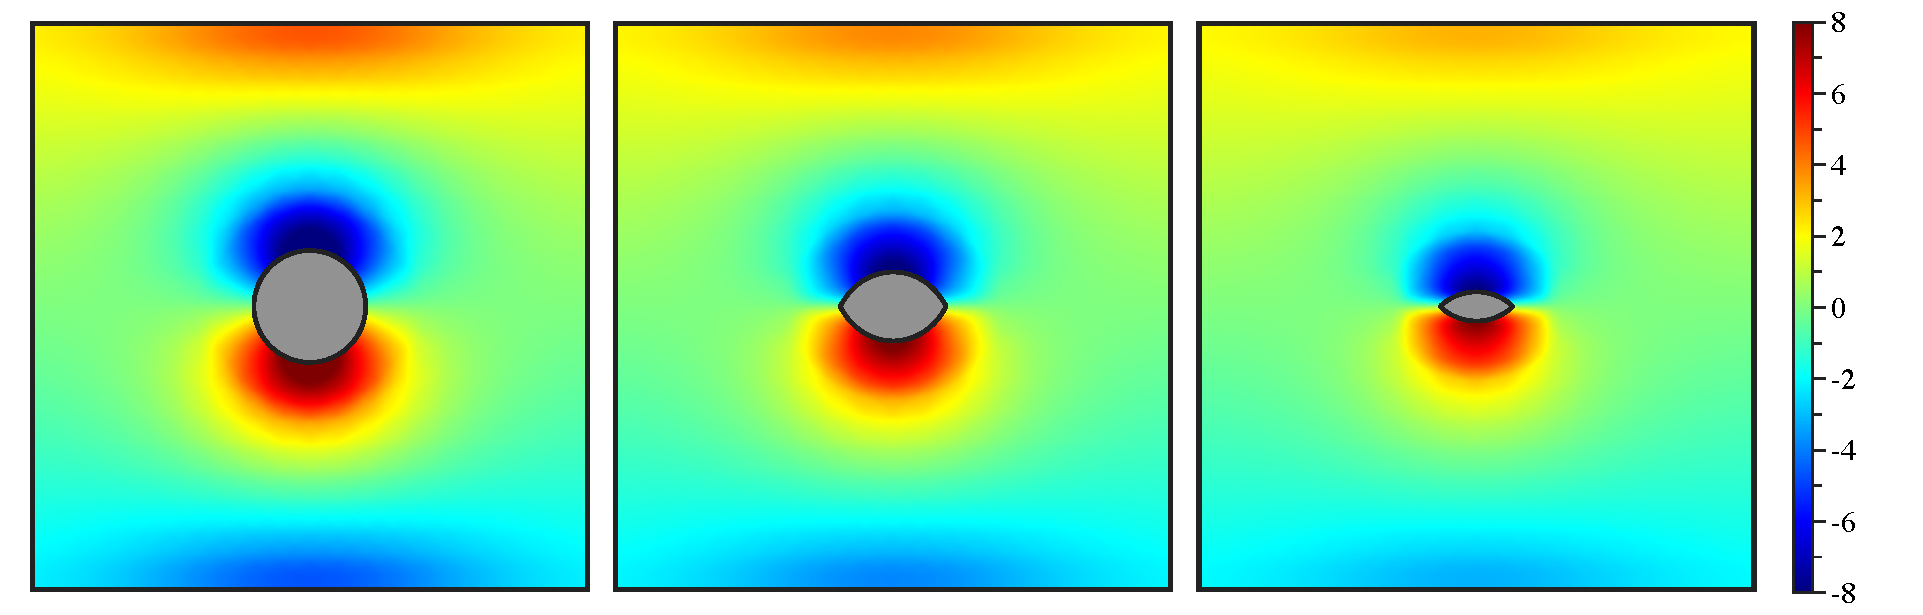
\includegraphics[width = 0.80 \textwidth]{./figs/01bodseq.pdf}
\caption{A single body eroding in Stokes flow. As the body erodes, it develops a corner at its front and rear stagnation points, while remaining for-aft symmetric due to time-reversibility. Color indicates the vorticity of the surrounding flow, which, when evaluated on the boundary, gives the local shear stress. In this simulation, we use $N_\iin = 1024$ discretization points on the body, $N_\out = 1024$ points on the outer boundary, a time-step of $\Dt = 10^{-6}$, and smoothing parameters of $\eps = 10/1024$ and $\sigma = 10/1024$.}
\label{01bodseq} 
\end{center}
\end{figure}
 %^^^^^^^^^^^^^^^^^^^^^^^^^^^^^^%
% Figure from datafile 01circ1024aa;
% Uses 01circ1024.in with epsfac = 10, sigfac = 10, dt = 1e-6, fixarea = 0, fixpdrop = 0

Figure \ref{01bodseq} shows the erosion of a single body, numerically simulated with $N_\iin = 1024$ discretization points and shown at three evenly spaced times. Here, color represents the vorticity of the surrounding flow. When evaluated on the boundary, vorticity corresponds to the shear stress and thus the local erosion rate. As seen in the left-most snapshot, the body is initially circular and has the strongest vorticity above and below it. The flow is for-aft symmetric as a result of the time-reversibility of the Stokes equations, with vorticity vanishing at the body's front and rear stagnation points. 
At the next instance, the body has lost material due to erosion, but remains for-aft symmetric due to the flow symmetry. The greatest material loss has occurred at the body's top and bottom, where shear is strongest. Interestingly, the body has developed well-defined corners at its front and rear stagnation points. This geometric feature is a consequence of the erosion law, which depends on the {\em absolute} shear stress: wherever the stress vanishes, $\atau$ exhibits a corner, which manifests as a corner in the geometry. As shown in the third snapshot, this corner persists as the bodies becomes even more slender and continues to shrink.

To better understand the shape evolution, Fig.~\ref{shrink_intface}(a) shows several superimposed interfaces at evenly spaced times. The interfaces are color-coded by normalized time $t/t_f$, where $t_f = 1.79 \times 10^{-2}$ is the time at which the body vanishes in the simulation. As seen in Fig.~\ref{shrink_intface}(a), the body converges to a fairly slender, for-aft symmetric shape that has corners at its front and back --- somewhat reminiscent of an American football.
Fig.~\ref{shrink_intface}(b) shows how the absolute shear stress, $\atau$, is distributed along each of these interfaces. The normalized arclength $s/L$ runs counterclockwise around the body, with $s/L = $ 0 and 0.5 corresponding to the rear and front stagnation points respectively. At early times (yellow curves), the stress varies significantly, with more stress concentrated at the top and bottom of the body. However, as erosion alters the body's shape, the stress becomes more uniformly distributed over the entire surface (red curves). The absolute stress $\atau$ shows slight peaks near the stagnation points as the bodies nears the final stages of erosion (dark red). Closer inspection reveals that the stress actually vanishes {\em at} the stagnation points, but in a region that becomes increasingly narrow with time.


%^^^^^^^^^^^^^^^^^^^^^^^^^^^^^^%
\begin{figure}%[htbp]
\begin{center}
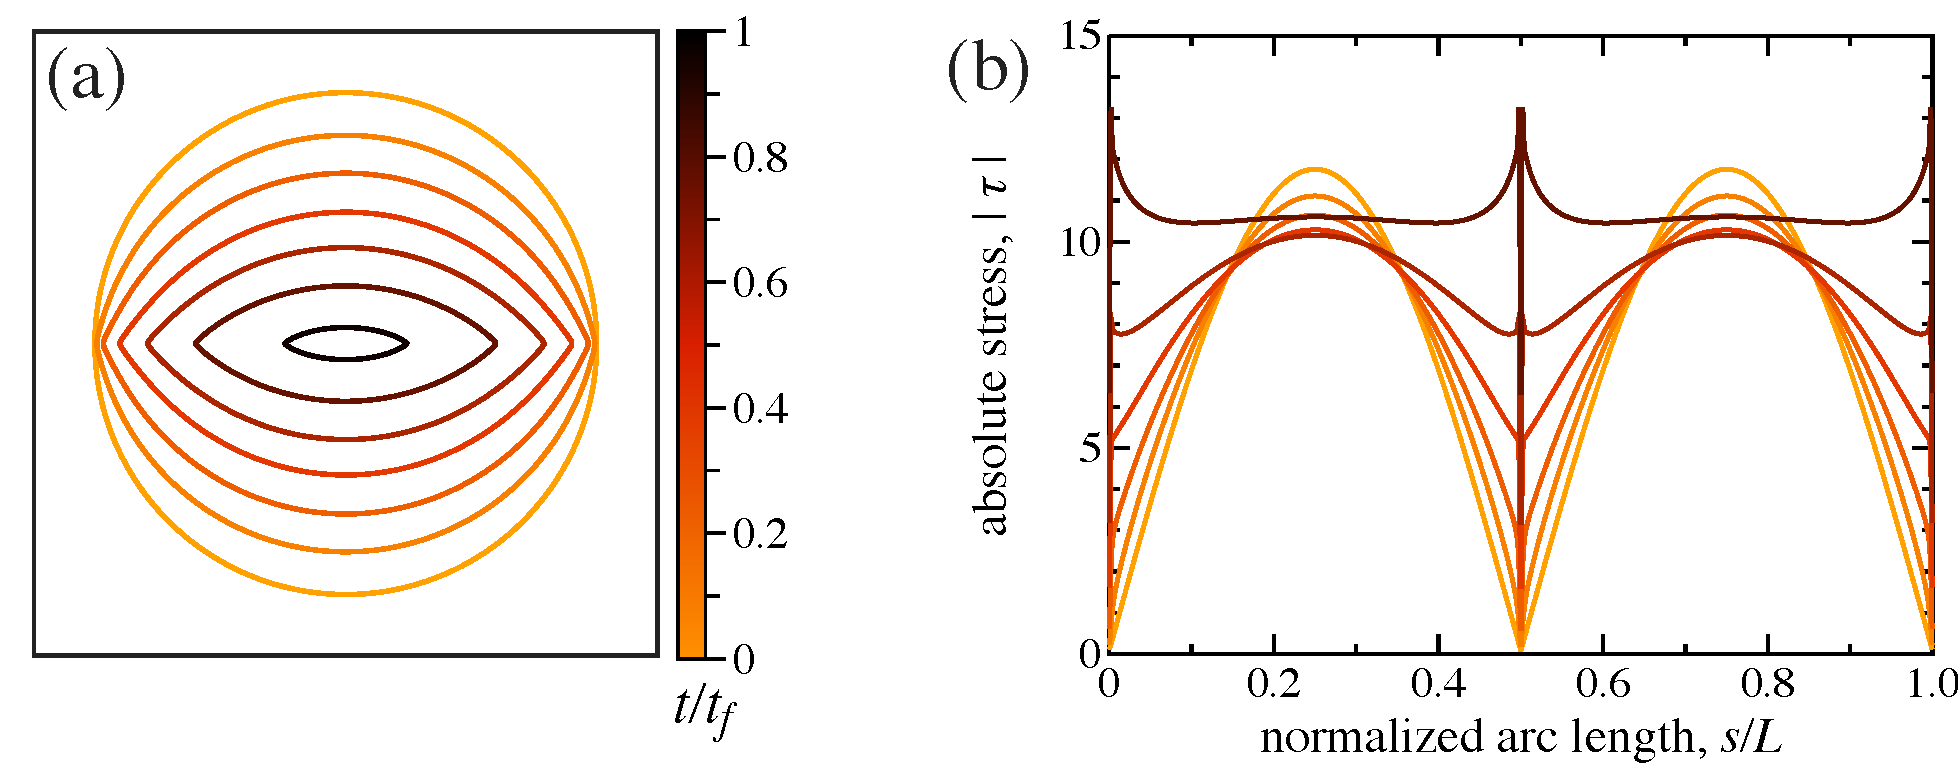
\includegraphics[width = 0.8 \textwidth]{./figs/shrink_intface.pdf}
\caption{
Shape and stress evolution: (a) Interfaces of the eroding body from Fig.~\ref{01bodseq} shown at evenly-spaced time intervals. Color indicates normalized time, $t/t_f$, where $t_f = 1.79 \times 10^{-2}$ is the time at which the body completely vanishes. (b) The distribution of absolute shear stress, $\atau$, along each of these interfaces. Normalized arclength, $s/L$, runs counterclockwise from the rear stagnation point. The stress initially varies over the body's surface, but becomes more uniform over time.}
\label{shrink_intface}
\end{center}
\end{figure}
 %^^^^^^^^^^^^^^^^^^^^^^^^^^^^^^%
% Figure from datafile 01circ1024aa;
% Uses 01circ1024.in with epsfac = 10, sigfac = 10, dt = 1e-6, fixarea = 0, fixpdrop = 0

\subsection{Scaling laws for area and drag}
\label{sec:scaling}

Figure~\ref{shrink_intface}(a) shows that the spacing between successive interfaces becomes larger with time, suggesting that the overall shear stress grows as the body vanishes. This observation is consistent with the well-known 3D Stokes drag law, in which stress, $\tau \sim \mu \umax / a$, scales inversely proportional to body-scale $a$ (e.g.~for a sphere, $a$ is the radius). This law must be modified in two dimensions, though. The modification is made non-trivial by subtleties of the 2D Stokes paradox, but can be correctly deduced by noting that, as the body vanishes, its drag must be consistent with slender-body theory \cite{batchelor1970slender, MooreJFM2012}. 
For a slender body in flow perpendicular to its long-axis $\ell$, the drag is proportional to
$\mu \umax \ell/ \log(\ell/a)$, where $a \ll \ell $ is a length scale of the cross-section. This law implies that the stress-per-unit-span on a 2D cross-section is approximately
\begin{align}
  \label{eqn:stresslaw}
  \tau \sim \frac{\mu \umax}{a \log(\ell/a)} \qquad \text{for } a \ll \ell \, .
\end{align}
In interpreting our 2D simulations, we will treat the span, $\ell$, as
fixed. Recall that $L$ denotes the total perimeter of the 2D cross-section. Since $L$ and $a$ each represent a characteristic scale of the cross-section, they can often be interchanged in scaling analysis.

%^^^^^^^^^^^^^^^^^^^^^^^^^^^^^^%
\begin{figure}%[htbp]
\begin{center}
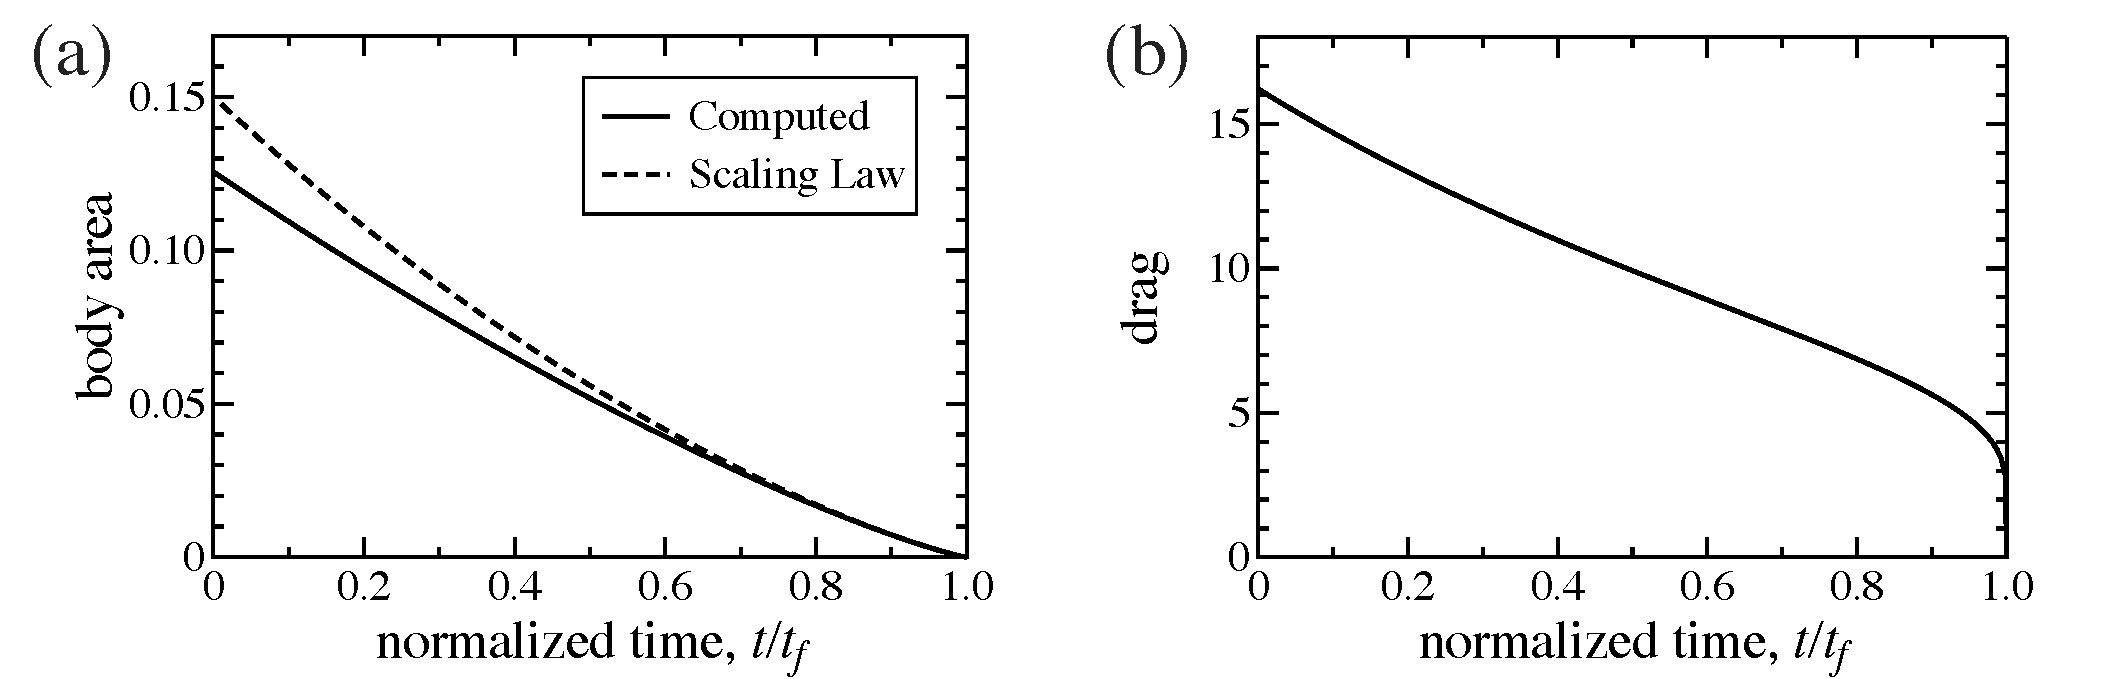
\includegraphics[width = 0.9 \textwidth]{./figs/area_drag.pdf}
\caption{Area and drag: (a) The body area measured in the simulations (black) shown against the scaling-law prediction~\eqref{area_predict} (dotted red), the two of which agree closely. (b) The horizontal drag (black) on the body as it erodes, along with the viscous (green) and pressure (blue) contributions. The scaling prediction can be rearranged to give estimate~\eqref{dragscaling} for the viscous drag (dotted red).}
\label{area_drag}
\end{center}
\end{figure}
 %^^^^^^^^^^^^^^^^^^^^^^^^^^^^^^%
% Figure from datafile 01circ1024aaa;
% Uses 01circ1024.in with epsfac = 10, sigfac = 10, dt = 1e-7, fixarea = 0, fixpdrop = 0

The body's rate of area reduction is given by integrating the absolute shear stress around the boundary
\begin{align}
\dot{A} = - \int_{\gamma} \atau \, ds \,  = - \mean{\atau} L \, ,
\end{align}
Thus, the rate of area reduction is given by the product of the mean shear stress $\mean{\atau}$ and the perimeter $L$, which is an {\em exact} relation. Inserting scaling law~\eqref{eqn:stresslaw} gives the estimate
\begin{align}
\dot{A} \sim \frac{ - \mu \umax}{\log(\ell/a)} \qquad \text{as } a \to 0 \, . 
\end{align}
Noting that $A \sim a^2$ allows one to solve the ODE, giving
\begin{align}
\label{area_predict}
\frac{A}{A_0} \left( 1 - c_1 \log{\frac{A}{A_0}} \right) \sim \frac{t_f - t}{t_f} \quad \text{as } t \to t_f \, .
\end{align}
Here, $t_f$ is the time of vanishing, $A_0$ is the body's initial area, and $c_1$ is a free constant. The above is an {\em implicit} relationship for how area scales down in time, and we can use this prediction to test our numerical simulation. In Fig.~\ref{area_drag}(a) we compare the area measured in our numerical simulation (black curve) against the above scaling law (red dotted curve) with $c_1 = 0.24$ a fit parameter. The two agree remarkable well throughout the entire simulation, thus co-validating the simulation and asymptotic results.

	As the body shrinks in accordance with \eqref{area_predict}, the drag that it exerts decreases at a related rate, which offers a second check on our numerics. In Fig.~\ref{area_drag}(b), we show the horizontal drag on the simulated body as it erodes (black curve). The drag, $F_D$, is calculated using \eqref{eqn:drag} and, in the context of slender-body theory, should be interpreted as the drag-per-unit-span on a 2D cross-section. As seen in the figure, $F_D$ decreases gradually at first, then abruptly tends to zero in the final moments as the vanishes. This behavior, though perhaps surprising, is consistent with the fact that drag vanishes {\em logarithmically} with body-size in 2D Stokes flow. Equation \eqref{eqn:drag} also allows us to calculate the separate contributions of pressure and viscous drag, and we show these with the blue and green curves in Fig.~\ref{area_drag}(b). Initially, pressure and viscous drag are comparable, with the circular geometry having a slightly higher level of pressure drag. As the body erodes and assumes a more slender form, though, the pressure drag decreases much more rapidly, leaving viscous drag to dominate. This behavior is associated with the tendency towards a drag-minimizing profile, which will be discussed in Section \ref{LimitingShape}.

As a check on these results, we can use slender-body theory to estimate the drag-per-unit-span
\begin{align}
\label{dragscaling}
\frac{F_D}{4 \pi} \sim \frac{ \mu U}{\log(\ell/a)}	\qquad \text{for } a \ll \ell \, .
\end{align}
For the case of a {\em circular} cylinder, the normalization factor of $4 \pi$ produces an {\em exact} relationship (under the slender-body assumptions), where $a$ is taken to be the radius. For other shapes the formula will be approximate and we define $a = \sqrt{A/\pi}$ as the characteristic lengthscale since it generalizes the case of a circle. In Fig.~\ref{area_drag}(b) we show this scaling prediction (red dotted curve), where $\ell = 2.3 a_0$ is a fit parameter and $a_0 = 0.2$ is the radius of the initially circular body. The scaling law and measured drag agree closely as $t \to t_f$, thus confirming that our simulation accurately captures the slender-body limit as the shape disappears.


\subsection{Local analysis for the limiting shape}
\label{LimitingShape}
 
With the vanishing rate understood, we now seek to quantify the limiting shape observed in Fig.~\ref{shrink_intface}(a). Certain features of this shape can be predicted analytically by appealing to the principal that, in long time, the shear stress becomes uniformly distributed along the body. In particular, consider the angle formed at the front and rear stagnation points. In a small region around this point, we can neglect body curvature and consider the problem of Stokes flow around an infinite wedge of opening angle $\oangle$. See Fig.~\ref{corner} for a schematic. This problem can be solved exactly in polar coordinates $(r, \theta)$ where $\theta \in [-\thb,\thb]$ and $\thb = \pi - \oangle/2$. (In this section alone, $\theta$ denotes the polar coordinate and not the local tangent angle). 

%^^^^^^^^^^^^^^^^^^^^^^^^^^^^^^%
\begin{figure}%[htbp]
\begin{center}
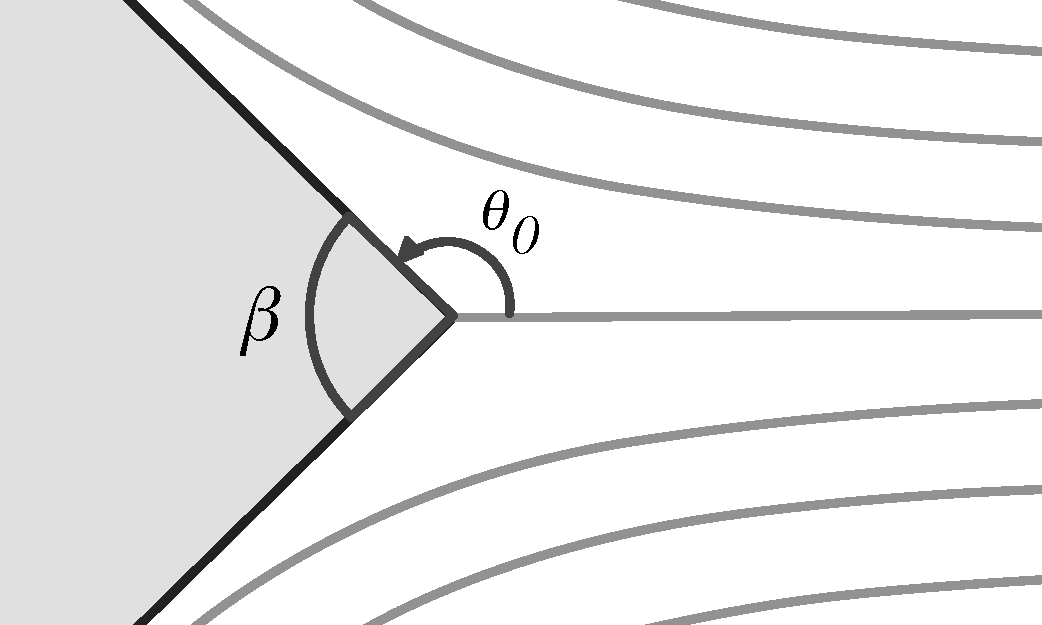
\includegraphics[width = 0.4 \textwidth]{./figs/corner.pdf}
\caption{Schematic of 2D Stokes flow near a corner: The flow around an infinite wedge of opening angle $\oangle$ is described by a stream-function $\psi(r,\theta)$ for $\theta \in [-\theta_0, \theta_0]$}.
\label{corner}
\end{center}
\end{figure}
 %^^^^^^^^^^^^^^^^^^^^^^^^^^^^^^%
 
The corresponding stream function is biharmonic, $\Delta^2 \psi = 0$, and the ansatz $\psi = r^{\lambda}f(\theta)$ gives the 4th-order ODE~\cite{poz1997}
\begin{align}
\label{fODE}
f'''' + 2(\lambda^2 - 2 \lambda + 2)f'' + \lambda^2(\lambda-2)^2 f = 0.
\end{align}
This ODE is subject to no-slip boundary conditions along the wedge $f(\thb) = f'(\thb) = 0$ and odd symmetry about the horizontal axis, $f(0) = f''(0) = 0$. For arbitrary opening angle $\beta$, ODE \eqref{fODE} and its boundary conditions constitute an eigenvalue problem for $\lambda$, whose solution furnishes the stream function and the corresponding shear stress on the wedge surface $\tau = \mu r^{\lambda-2} f''(\thb)$. We, however, seek to determine the particular opening angle that produces {\em uniform} shear stress and thus set $\lambda = 2$. The corresponding solution to \eqref{fODE} that satisfies odd symmetry is given by
\begin{align}
  f(\theta) = B \sin (2 \theta) + C \theta \, ,
\end{align}
and imposing the no-slip boundary conditions gives the condition
\begin{align}
  \sin(2 \thb) - 2 \thb \cos(2 \thb) = 0 \, .
\end{align}
This nonlinear equation has solution $\thb \approx 129^\circ$, which gives the uniform-stress opening angle as $\oangle \approx 102^\circ$ degrees. 
% Pozrikidis page 239: symmetric flow.

\todo[inline]{Here in revising}

We note that this uniform-stress shape is closely related to the so-called `optimal profile in Stokes flow' found by Pironneau (1973) \cite{pir1973}, who determined the shape that minimizes drag in 3D Stokes flow subject to the constraint of fixed volume (see also \cite{mon-lau2015} for an interesting related shape). Pironneau's 3D shape has an opening angle of $120^{\circ}$ and ours is simply the 2D counterpart with its slightly different $102^{\circ}$ opening angle. Previous numerical simulations on erosion in 3D Stokes flow revealed that, in long time, an eroding body tends to a shape that is approximately (though not precisely) Pironneau's optimal profile \cite{mit-spa2016}.


\subsection{Fixed-area simulations}

%^^^^^^^^^^^^^^^^^^^^^^^^^^^^^^%
\begin{figure}%[htbp]
\begin{center}
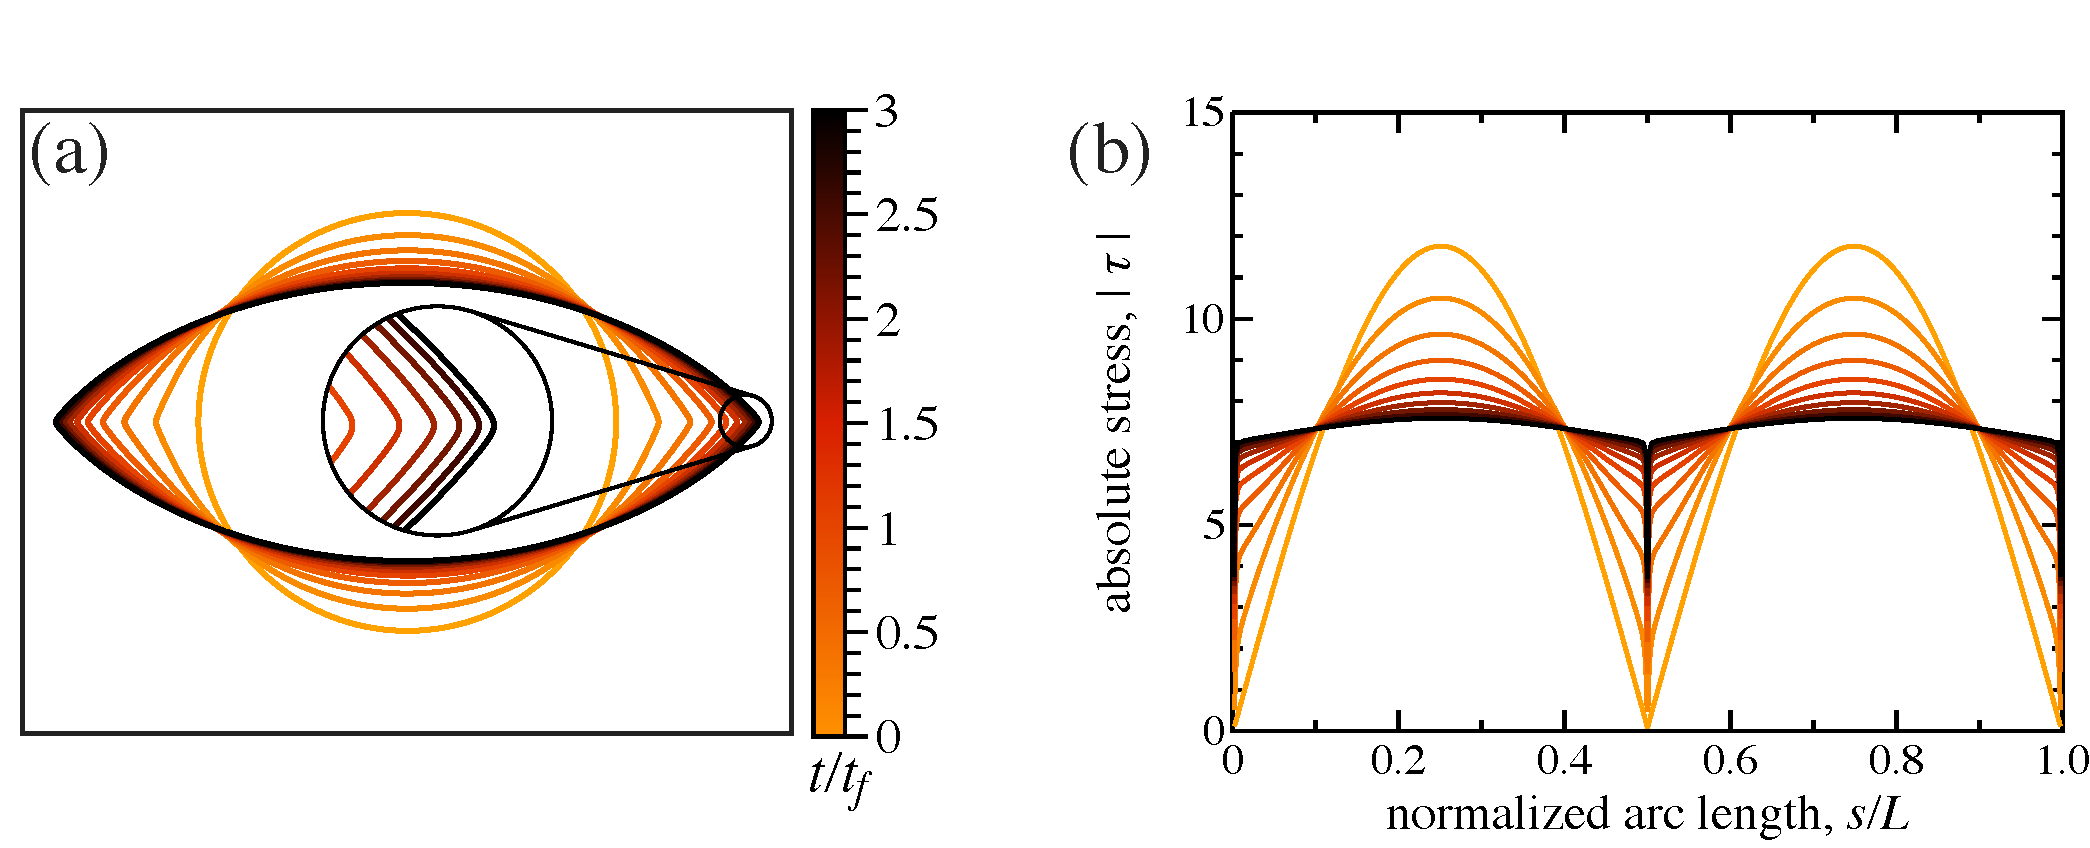
\includegraphics[width = 0.85 \textwidth]{./figs/fixed_intface.pdf}
\caption{Fixed-area simulations: (a) Interfaces of a body eroding under shear stress but with the area artificially kept constant. Inset: zoom near the rear stagnation point, showing that the corner is actually smooth on a fine scale. (b) The shear-stress distribution on each of these interfaces. As the body erodes and converges to a terminal form, the stress becomes more uniformly distributed over the entire surface.}
\label{fixed_intface}
\end{center}
\end{figure}
 %^^^^^^^^^^^^^^^^^^^^^^^^^^^^^^%
% Figure from datafile 01circ1024c5
% Uses 01circ1024.in with epsfac = 5, sigfac = 5, dt = 2e-4, fixarea = 1, fixpdrop = 0

To compare with this analytical prediction, we aim to measure the opening angles formed in our numerical simulations. Section \ref{sec:scaling}, however, shows that the magnitude of the shear stress diverges as the body vanishes, which causes our simulations lose accuracy just in the final critical moments when the body is expected to approach its limiting shape. To circumvent this problem, we remove the effect of shrinking by forcing $\Vn$ to have zero mean,
\begin{align}
\Vn \leftarrow \Vn - \mean{\Vn} \, .
\end{align}
This modification allows erosion to sculpt the shape as it would normally, but with the area artificially held fixed.

	We show in Fig.~\ref{fixed_intface}(a) several interfaces of this modified erosion process. Notice the body obtains a similar profile as observed previously, but with fixed area. Importantly, more numerical accuracy is now available to quantify the terminal state. The inset in Fig.~\ref{fixed_intface}(a) shows a zoom of the body's rear stagnation point, demonstrating that the near-corner is actually smooth on a fine scale, in accordance with our numerical smoothing. 
Likewise, Fig.~\ref{fixed_intface}(b) shows the stress distribution on the evolving body, revealing that stress becomes more uniform as time proceeds. Interestingly, the slight rise in shear near the front/rear corners that was seen in Fig.~\ref{shrink_intface}(b) is no longer present, suggesting that the effect was due to loss of accuracy. Here, time is normalized by the same vanishing time $t_f = 1.79 \times 10^{-2}$ as in Fig.~\ref{shrink_intface}. Curiously, about 3 multiples of $t_f$ are required to reach an approximate steady-state. This contrasts with previous studies of high-Reynolds-number erosion, in which a satisfactory steady-state was usually reached before the body vanished~\cite{moo-ris-chi-zha-she2013}.

%^^^^^^^^^^^^^^^^^^^^^^^^^^^^^^%
\begin{figure}%[htbp]
\begin{center}
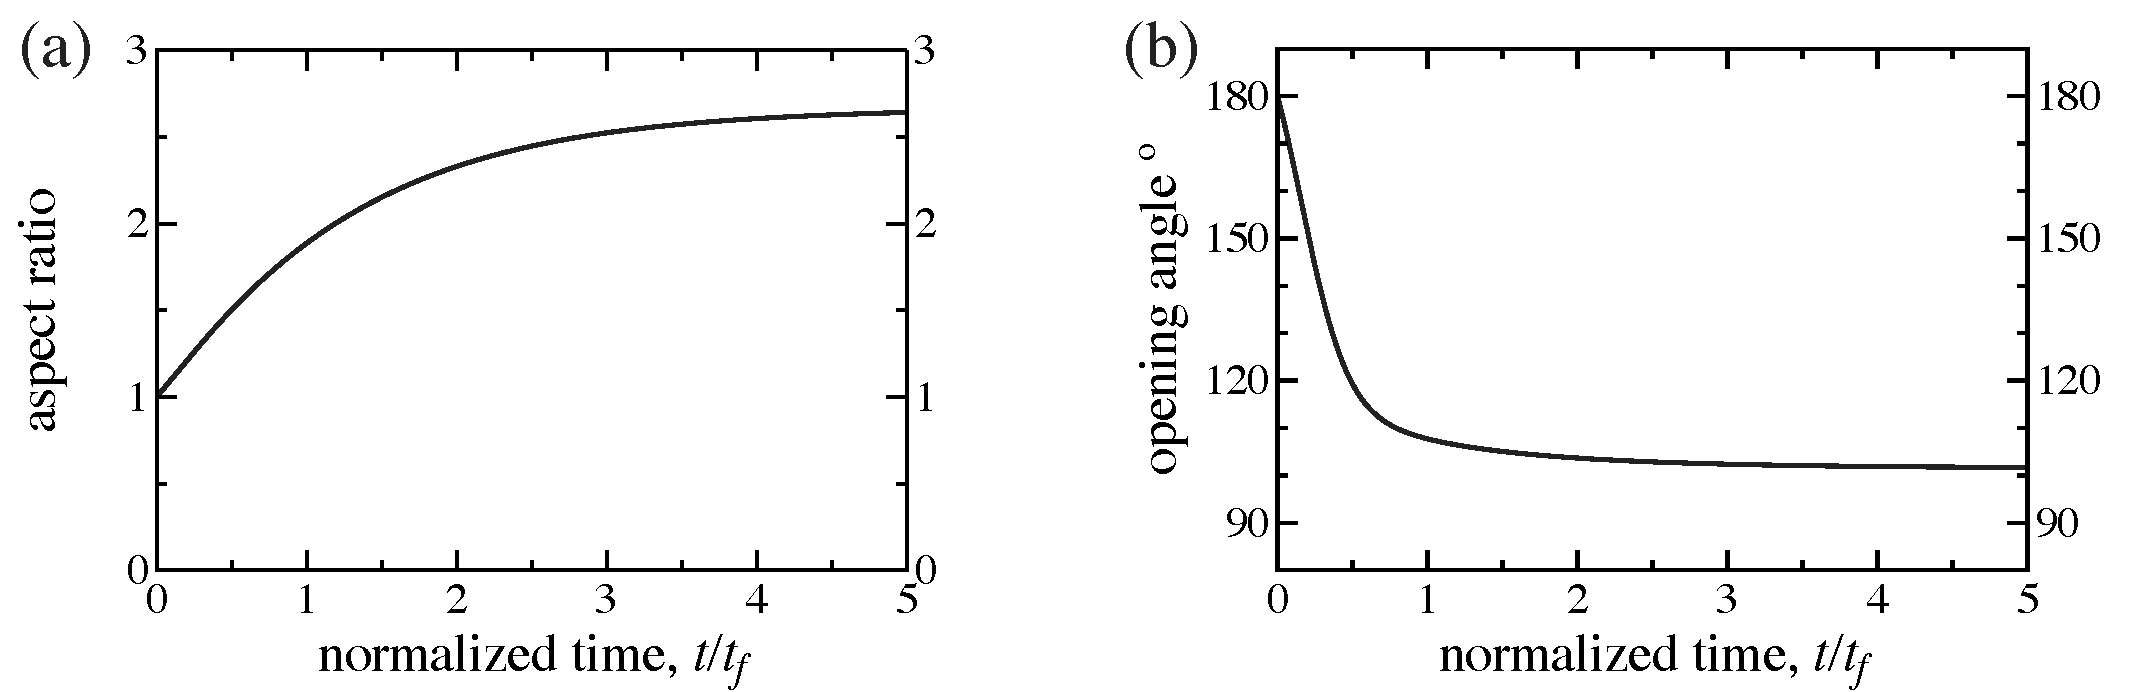
\includegraphics[width = 0.85 \textwidth]{./figs/arangle.pdf}
\caption{Shape characteristics of an eroding body: (a) The aspect ratio, defined as the width to height, versus time. (b) The measured opening angle versus time. For both measurements, we show three cases of the smoothing parameters: $\eps = \sigma = 20/1024, 10/1024,$ and 5/1024. In the most resolved simulation (5/1024) the aspect ratio converges to 2.7 and the opening angle converges to the predicted value of $102^{\circ}$ in long time.}
\label{fig:arangle}
\end{center}
\end{figure}
 %^^^^^^^^^^^^^^^^^^^^^^^^^^^^^^%
% Figure from datafile 01circ1024c5
% Uses 01circ1024.in with epsfac = 5, sigfac = 5, dt = 2e-4, fixarea = 1, fixpdrop = 0

The fixed-area simulations allow for us to precisely measure characteristics of the shape. In particular, Fig.~\ref{fig:arangle} shows measurements of the body's aspect ratio (its width to height) and the front opening angle as they vary in time. We show these measurements for three simulations in which the smoothing parameters, $\eps$ and $\sigma$, are sequentially reduced, allowing us to assess convergence in these parameters. As shown in Fig.~\ref{fig:arangle}(a), the aspect ratio begins at one for the initial circular geometry and increases in time as erosion sculpts a more slender shape. The aspect ratio reaches a long time limit of about 2.7 in the most resolved simulation. Fig.~\ref{fig:arangle}b shows the body's opening angle, which we measure by fitting the tangent angle $\theta(\alpha)$ with a 7th degree polynomial over a region excluding the front/rear stagnation point (where a near-corner is approximated by a smooth curve of very high curvature). The polynomial fit is then extrapolated to the stagnation point to obtain an angle estimate (subject to some uncertainty, which we estimate below). As seen in Fig.~\ref{fig:arangle}a, the opening angle is initially $180^\circ$, corresponding to the initially circular geometry. Erosion causes the angle to form after a short time, and the angle becomes increasingly sharp as it converges to the value $102^\circ$ in the most resolved simulation. This coincides exactly with the valued predicted by our local solutions.

To examine the influence of the smoothing parameters, $\eps$ and
$\sigma$, we show in Table~\ref{table:arangle} the measurements of the
aspect ratio and the opening angle for different simulations. We fix the total number of discretization points at $N_\iin = 1024$ and sequentially reduce the smoothing with $\eps$ and $\sigma$ always equal. We choose the values $20/1024$, $10/1024$, and $5/1024$. 
Loosely, this corresponds to smoothing over the nearest 20, 10, and 5 grid points respectively. As seen in the table, the aspect ratio converges to a values of $2.65$ and the opening angle converges to $102^{\circ}$. We also estimate the uncertainty in the angle measurements by varying the region of the polynomial fit and the degree of the fit. As shown in the table, as the smoothing parameters are reduced, the angle measurements become more precise.

% Table
%^^^^^^^^^^^^^^^^^^^^^^^^^^^^^^%
\begin{table}%[htbp]
\begin{center}
\caption{Final aspect ratio and opening angle
} 
\vspace{0.3 pc}
\label{table:arangle}
\begin{tabular}{c c c}
\hline
\hspace{0.5pc} smoothing parameters: $\eps$ and $\sigma$
\hspace{0.5pc} & final aspect ratio 
\hspace{0.5pc} & final opening angle \\
\hline
20/1024		& 2.55	& $110^\circ \pm 6^\circ$	\\
10/1024		& 2.62	& $104^\circ \pm 4^\circ$	\\
5/1024		& 2.65	& $102^\circ \pm 2^\circ$	\\
\hline
\end{tabular}
\end{center}
\end{table}
 %^^^^^^^^^^^^^^^^^^^^^^^^^^^^^^%
% npts = 1024


\subsection{Convergence test}

As a final validation, we now aim to verify that our method converges with second-order accuracy in time. To this end, we run the same single-body simulation from Figs.~\ref{01bodseq} and \ref{shrink_intface} (except with a coarser $N_\iin=256$) to a stopping time of $t_s = 10^{-2}$. This stopping time is 56\% of the time it takes the body to vanish, and was selected so that the body will have eroded substantially but is not so small that accuracy is compromised. We assess error by measuring the difference between simulations of successive resolutions (i.e.~we verify Cauchy convergence). In particular, we measure the $L^2$-difference of the body shapes obtained at the stopping time. At each stage we halve the timestep $\Delta t$. Table \ref{convtab} shows the $L^2$-errors between successive simulations, along with the order of accuracy as obtained by Richardson-extrapolation-type calculations. The table confirms that our method to converges with second-order accuracy. In the table, we also show the CPU time of the simulation run on a single processor (though the algorithm is easily parallelized), showing a linear increase in computational time.

% Table
%^^^^^^^^^^^^^^^^^^^^^^^^^^^^^^%
\begin{table}%[htbp]
\begin{center}
\caption{Convergence test: We run single-body erosion simulations to a stopping time of $t_s = 10^{-2}$ (56\% of the vanishing time) and measure the $L^2$-difference in shapes obtained with successive temporal resolutions. The tests confirm the method to be second-order accurate in time. The last column shows the measured CPU time which increases linearly as the time-step is refined.
}
\vspace{0.3 pc}
\label{convtab}
\begin{tabular}{l l l l}
\hline
\hspace{0.0pc} $\Delta t/t_s$
\hspace{0.5pc} & error 
\hspace{0.5pc} & order
\hspace{0.5pc} & CPU time \\
\hline
%
1/50		& 1.68E-5		& --		& 53 secs     	\\
1/100	& 4.84E-6		& 1.79	& 1.8 mins   	\\
1/200	& 1.30E-6		& 1.90	& 3.5 mins  	\\
1/400	& 3.36E-7		& 1.95	& 6.9 mins  	\\
1/800	& 8.54E-8		& 1.98	& 14 mins   	\\
1/1600	& 2.15E-8		& 1.99	& 28 mins  	\\
1/3200	& 5.40E-9		& 1.99	& 56 mins    	\\
1/6400	& --			& --		& 111 mins	\\
%
\hline
\end{tabular}
\end{center}
\end{table}
 %^^^^^^^^^^^^^^^^^^^^^^^^^^^^^^%
% Parameters in this test are: 01circ256, nits = 7, dt0 = 1e-4, tfin = 1e-2
% epsfac = 10, sigfac = 10, fixarea = 0, fixprdop = 0


\section{Results: Multi-body erosion}
\label{s:MultiResults}

\subsection{Fixed pressure drop condition and validation}

With the numerical method validated, we are now ready to simulate the erosion of multiple bodies. We make one important conceptual change to our model. For a realistic porous medium composed of many solid bodies, the condition of a fixed incoming flow rate, $\umax$, is somewhat artificial. A more realistic condition is that the pressure difference from one end to another is held fixed. For example, in groundwater flow, this condition would correspond to a recharge region of given hydraulic head connecting to a discharge region of another hydraulic head. 

We therefore impose the condition of a fixed pressure difference by dynamically controlling the incoming flow-rate, $\umax$. This is achieved by first computing the Stokes flow with $\umax = 1$ prescribed, then measuring the pressure at a location upstream ($x = -2$) and downstream ($x=2$) of the eroding bodies. The vertically-averaged upstream and downstream pressures are given by
\begin{align}
p_{-} = \frac{1}{2} \int_{-1}^{1} p(-2,y) \, dy \, , \qquad
p_{+} = \frac{1}{2} \int_{-1}^{1} p(+2,y) \, dy \, .
\end{align}
We then rescale the computed density function by the pressure difference
\begin{align}
\eeta \leftarrow \frac{\eeta}{(p_{-} - p_{+})} \, .
\end{align}
This rescaling maintains a {\em fixed} pressure difference between the upstream ($x=-2$) and downstream ($x=2$) positions. Because the Stokes equations are linear, such a rescaling is permissible and does not alter the accuracy of our method. Furthermore, {\em dynamic} rescaling is also permissible because the Stokes equations are memoryless (i.e.~there is no time derivative present in the PDEs).

%^^^^^^^^^^^^^^^^^^^^^^^^^^^^^^%
\begin{table}%[htbp]
\begin{center}
\caption{Convergence test for multiple-body erosion with fixed-pressure-drop condition. In this test, we use 20 bodies with $N_{\iin} = 128$ grid points on each. We run the simulations to a stopping time of $t_s = 4 \times 10^{-3}$ (24\% of the time it takes for {\em all} bodies to vanish). We measure the {\em combined} $L^2$-difference in the shapes of {\em all} bodies. The table confirms that the method maintains second-order accuracy in time, even with multiple bodies and a time-varying inflow rate $\umax$.
%We compare the shapes of {\em all} bodies from simulations of successive resolution using {\combined} $L^2$-norm
}
\vspace{0.3 pc}
\label{convtab}
\begin{tabular}{l l l l}
\hline
\hspace{0.0pc} $\Delta t/t_s$
\hspace{0.5pc} & error 
\hspace{0.5pc} & order
\hspace{0.5pc} & CPU time \\
\hline
%
1/10     	& 2.67E-5  	& --        	& 14 mins  	\\
1/20     	& 7.23E-6  	& 1.88 	& 27 mins  	\\
1/40     	& 1.95E-6  	& 1.89 	& 52 mins  	\\
1/80     	& 4.90E-7  	& 1.99 	& 1.7 hours	\\
1/160     	& 1.25E-7  	& 1.97  	& 3.4 hours	\\
%
\hline
\end{tabular}
\end{center}
\end{table}
 %^^^^^^^^^^^^^^^^^^^^^^^^^^^^^^%
% Parameters in this test are: 20circ128, nits = 5, dt0 = 4e-4, tfin = 4e-3
% epsfac = 10, sigfac = 10, fixarea = 0, fixprdop = 1

Briefly, to verity that the rescaling does not alter accuracy, we show in Table \ref{convtab} a convergence test for a 20-body simulation with the condition of fixed pressure drop imposed. The table confirms that the method retains second-order accuracy in time. In the last column, we show the computational times, indicating that the 20-body simulations require more runtime than the single-body case. Although the GMRES-iteration count is independent of the spatial resolution, $N_{\iin}$, it can depend on the number of bodies and/or their configuration. To illustrate this point, we show in Table~\ref{itertab} the GMRES count for various cases ...
\todo[inline]{preconditioning papers are~\cite{qua-cou-dar2018}
and~\cite{qua-bir2015a}}

% Table: GMRES iterations
%^^^^^^^^^^^^^^^^^^^^^^^^^^^^^^%
\begin{table}%[htbp]
\begin{center}
\caption{GMRES Iterations: the tolerance is 1E-8.
}
\vspace{0.3 pc}
\label{itertab}
\begin{tabular}{c c | c c}
\hline
\hspace{0.5pc} Number of bodies
\hspace{0.5pc} & GMRES iterations 
\hspace{0.5pc} & Resolution, $N_{\iin}$
\hspace{0.5pc} & GMRES iterations  \\
\hspace{0.0pc} ($N_\iin = 128$ fixed) & 
\hspace{0.5pc} &(10 bodies) & \\
\hline
%
10	& 223	& 32	    	& 228	\\
15	& 292	& 64    	& 226	\\
20	& 363	& 128	& 223	\\
30	& 496	& 256	& 223	\\
40	& 676	& 512	& 223	\\
50	& 991	& 1024	& 223	\\
%
\hline
\end{tabular}
\end{center}
\end{table}
 %^^^^^^^^^^^^^^^^^^^^^^^^^^^^^^%
% In these tests I always use 128 points per body.

\subsection{Multi-body erosion}

We now discuss some physical aspects of multi-body erosion revealed by our simulations. Figure~\ref{fig:06bodies} shows a simulation of 6 eroding bodies, each initially circles of various sizes and positions. Over time, erosion not only diminishes the size of the bodies, but also alters their shapes considerable. As in the single-body simulations, corner-like features develop, but not in locations that are easily predictable. Rather, when and where these sharp features develop depends on inter-body feedback as mediated by the Stokes flow.

%^^^^^^^^^^^^^^^^^^^^^^^^^^^^^^%
\begin{figure}%[htbp]
\begin{center}
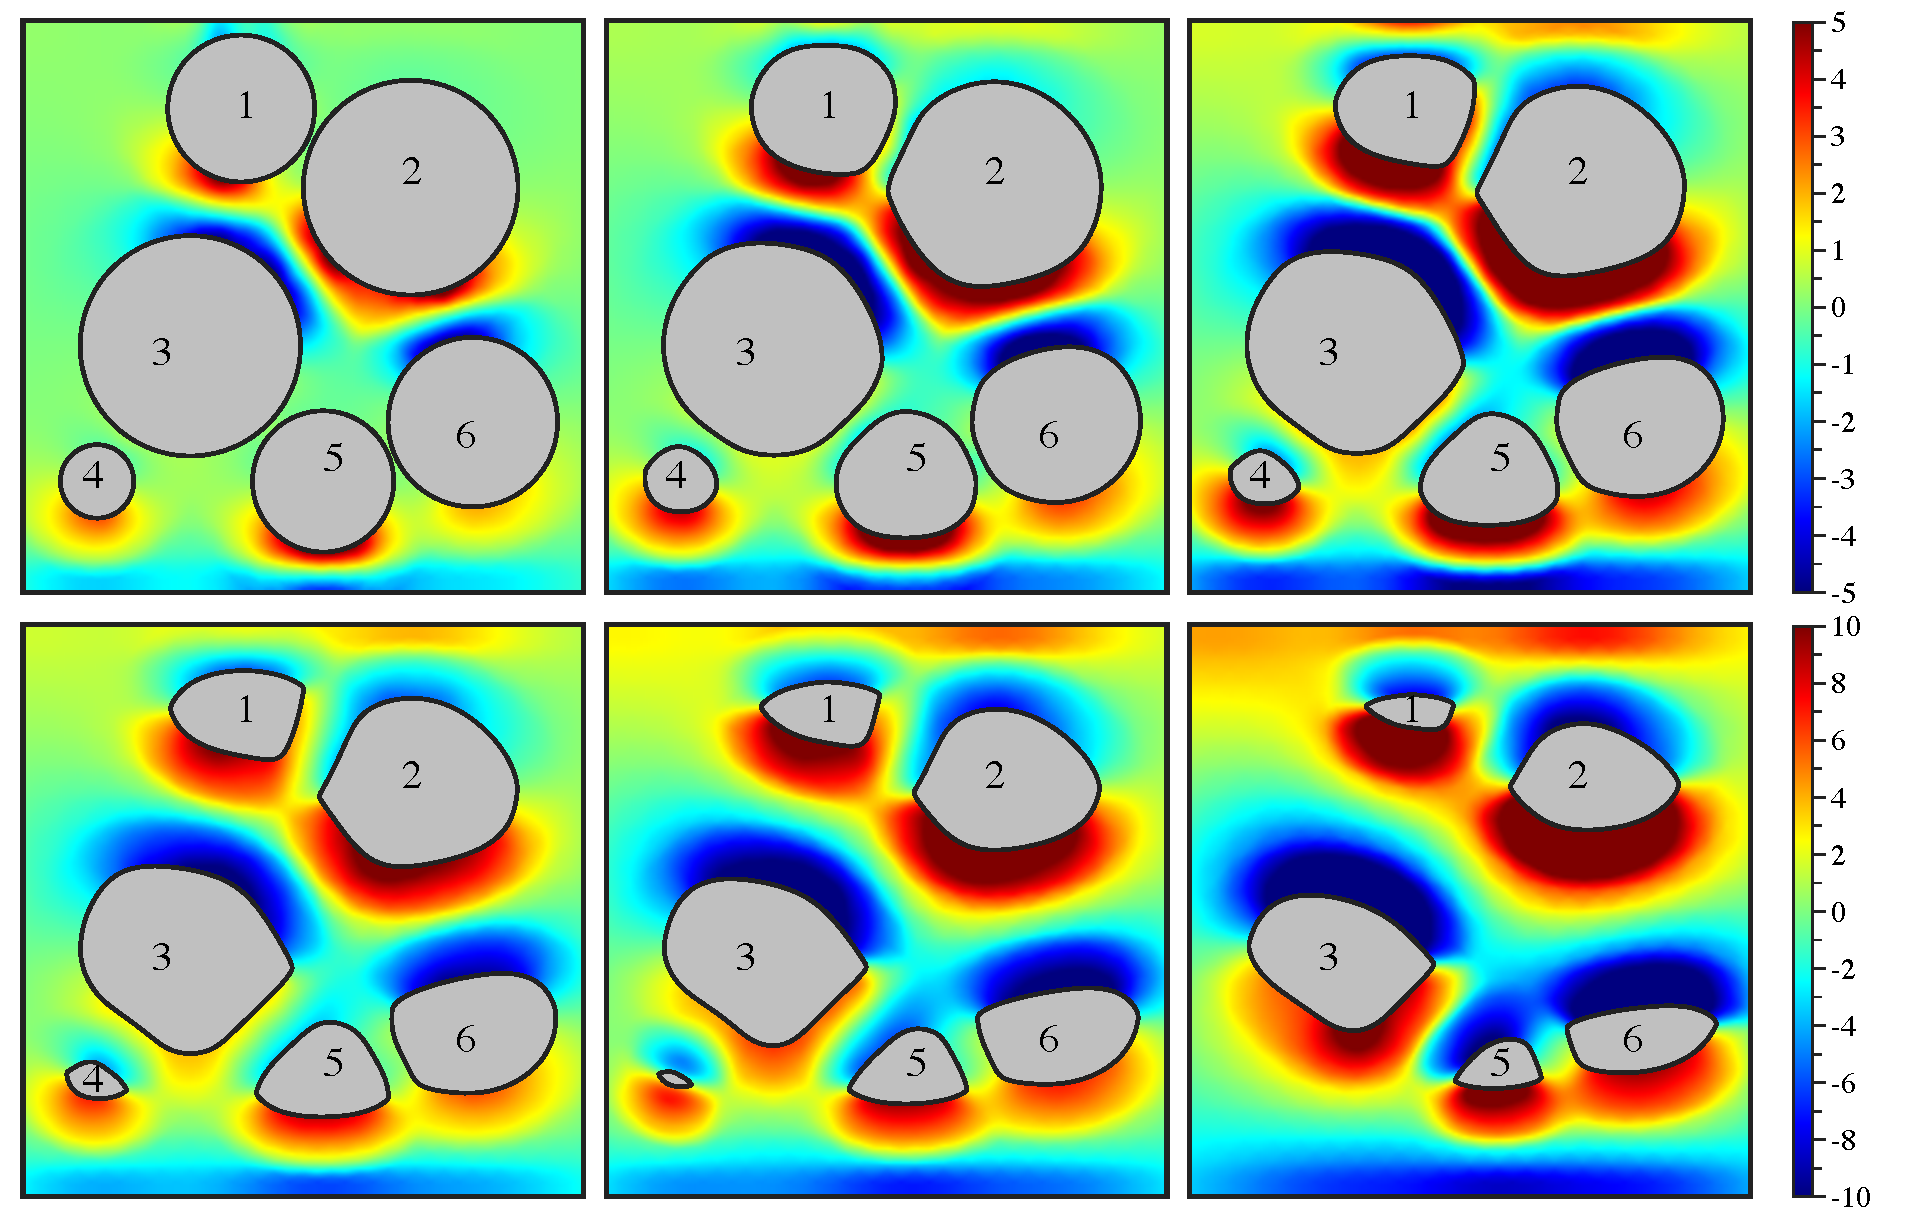
\includegraphics[width = 0.9 \textwidth]{./figs/06bod.pdf}
\caption{\label{fig:06bodies} 6 bodies.
}
%A time lapse of 50 bodies eroding in a viscous flow.  The boundary conditions are a constant pressure drop that creates a flow from the left to right.  The rate of erosion is proportional to the shear stress which is equivalent to the vorticity evaluated on the bodies.  The colors represent the vorticity, so regions with large vorticity (in magnitude) are regions where the flow will erode the fastest.
\end{center}
\end{figure}
 %^^^^^^^^^^^^^^^^^^^^^^^^^^^^^^%
% Figure generated from data file 50circ512p5, 
%which uses 50circ512.in with epsfac = 30, sigfac = 10, dt = 1e-4, fixpdrop = 1

The initial configuration in  Fig.~\ref{fig:06bodies} was selected to have several near contacts between bodies, for example between bodies 1 \& 2, 3 \& 5, and 5 \& 6. Our method handles these near contacts without difficulty. Interestingly, erosion appears to preferentially remove material from these regions of near contact, as the narrow spacing between bodies expands rather rapidly. For example, the spacing between bodies 1 \& 2 is initially very small, but by the second frame, is comparable to the spacing between bodies 3 \& 4. Even more interesting, the bodies tend to develop flat faces where there are near contacts. This effect leads to the appearance of straight channels in between bodies, for example between bodies 1 \& 2, 3 \& 5, and 5 \& 6. Once formed, these straight channels persist until the bodies have nearly vanished.

The vorticity field not only allows us to visualize regions of high shear, but also allows us to identify preferred channels with most intense flow. Figure~\ref{fig:06bodies} shows that the flow is concentrated primarily in a single channel that runs horizontally below bodies 1 \& 2 and above bodies 3, 5, \& 6. This main channel widens the fastest, and secondary channels follow (e.g.~between bodies 1 \& 2 or 3 \& 5 or 5 \& 6). Since the pressure drop across the cell is fixed, the overall flow rate increases as the bodies erode. This can be seen by the overall vorticity magnitude growing in time. By the final frame shown, body 4 has vanished completely and our method handles this event seamlessly.

%^^^^^^^^^^^^^^^^^^^^^^^^^^^^^^%
\begin{figure}%[htbp]
\begin{center}
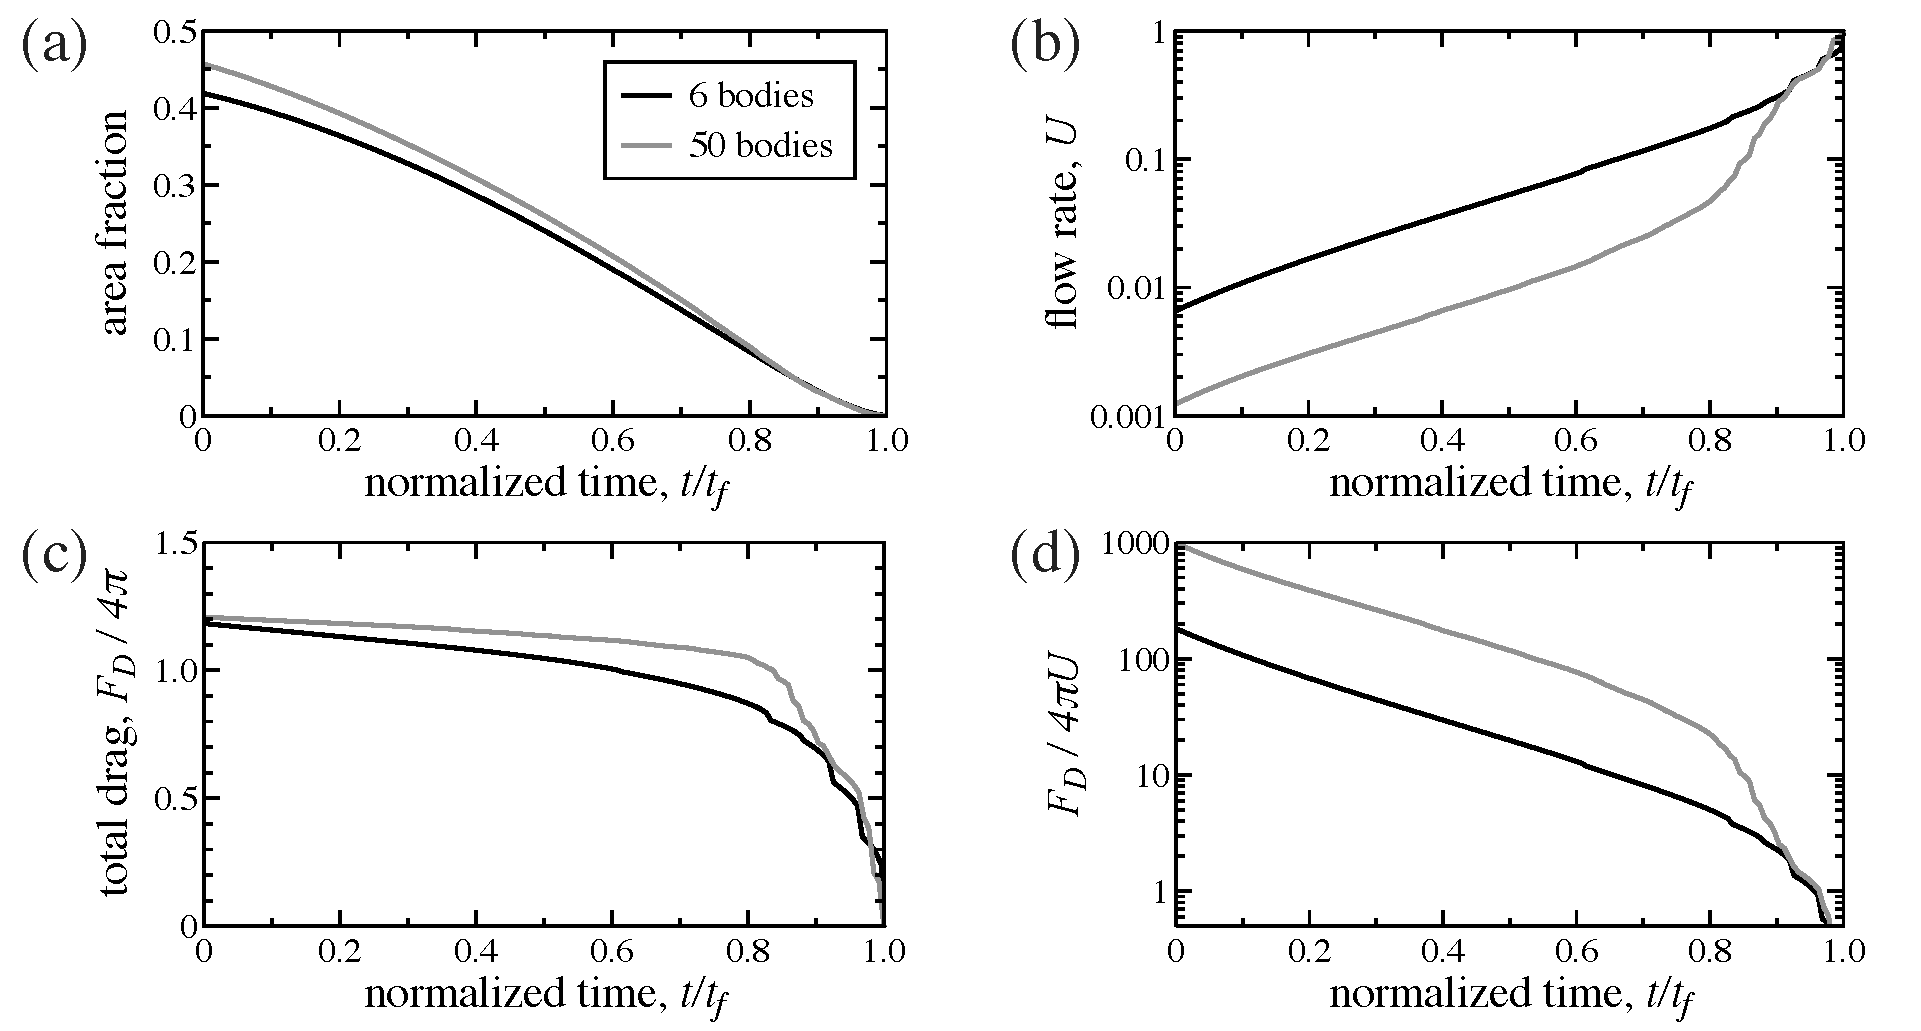
\includegraphics[width = 0.95 \textwidth]{./figs/mbodyplots.pdf}
\caption{\label{fig:mbodyplots} plots to go with 6 body simulation.
}
\end{center}
\end{figure}
 %^^^^^^^^^^^^^^^^^^^^^^^^^^^^^^%
% Figure generated from data file 50circ512p5, 
%which uses 50circ512.in with epsfac = 30, sigfac = 10, dt = 1e-4, fixpdrop = 1

We further quantify many of these observations in Fig.~\ref{fig:mbodyplots}. First, Fig.~\ref{fig:mbodyplots}(a) shows area fraction versus time. The area fraction is the total area of all bodies as compared to the domain area, i.e.~the 2D counterpart of volume fraction. The initial configuration of 6 circles comprises about 40\% of the domain area, and this percentage steadily decreases as the bodies erode. Figure \ref{fig:mbodyplots}(b) shows the inlet/outlet flow-rate, $\umax$, over time. Since we have fixed the pressure drop across the cell in these simulations, $\umax$ steadily increases as the bodies diminish and provide less resistance. Here, the vertical axis is logarithmic, and so the plot suggests exponential increase of $\umax$ at early times. This rapid increase in flow is likely due to the erosion-induced channelization observed above. In Fig.~\ref{fig:mbodyplots}(c) we show the total drag, summed over all bodies, versus time. Though the bodies diminish due to erosion, the steady increase of $\umax$ causes the total drag to remain relatively constant. Only near the end of the simulation does the drag decrease rapidly to zero. To remove the effect of increasing flow rate, we show in Fig.~\ref{fig:mbodyplots}(d) the total drag scaled on $\umax$. This value is a measure for the aggregate {\em resistance} of all bodies. Due to linearity of the Stokes equations, this measure does not depend on the flow-rate $\umax$, only on the bodies and their configuration. As seen here, the resistance decreases rapidly as the bodies erode. Since the vertical axis is logarithmic, the plot suggests an exponential decrease in resistance at early times, which is likely connected to the channelization process.

In Fig.~\ref{fig:mbodyplots} we also plot the same quantities for the 50-body simulation that was shown in Fig.~\ref{fig:50bodies} of the introduction. Overall, these plots support the same trends seen in the 6-body simulation. The initial area-fraction of the 50-body simulation is only slightly higher, about 45\%, and this fraction decreases steadily as bodies erode. The flow rate $\umax$ again increases very rapidly with time, though with a significantly smaller initial value due to the higher resistance provided by 50 bodies. As before, the total drag remains relatively constant throughout most of the simulation and then abruptly decreases to zero in the final moments. Our measure of resistance, $F_D/(4 \pi \umax)$, again decreases very rapidly in the early moments when channels are initially formed. Though the area fractions of the two simulations are nearly the same, the 50-body configuration provides about 5 times more resistance.


{\bf Good word: Spontaneous channelization}



%%%%%%%%%%%%%%%%%%%%%%%%%%%%%%%%%%%%%%%%%%%%%%%%%%%%%%%%%%%%%%%%%%%%%%%
\section{Conclusions\label{s:conclusions}}


%%%%%%%%%%%%%%%%%%%%%%%%%%%%%%%%%%%%%%%%%%%%%%%%%%%%%%%%%%%%%%%%%%%%%%%
\paragraph{\bf Acknowledgments} The authors would like to thank Manas
Rachh for supplying the FMM for the Stokes double-layer potential.


\todo[inline]{paper of Bryan, Eric, and Pieter and one with Pietro,
George, and Ruben}

\bibliographystyle{plainnat} 
\bibliography{refs}
\biboptions{sort&compress}
\end{document}


